\coursepart{2}{(MATH102) Calculus II}

% 2020 Fall KAIST Calculus II Midterm, Problem 1
\begin{problem}[2020 Fall \KAIST{} Calculus II]
A particle is located at the point $(2,-3)$ on a metal plate whose temperature is given by
\[
T(x,y)=20-4x^2-y^2.
\]
Find the directions of
\begin{problemsubparts}
\item the most rapid increase in temperature,
\item the most rapid decrease in temperature, and
\item the least change.
\end{problemsubparts}
\end{problem}

% 2020 Fall KAIST Calculus II Midterm, Problem 2
\begin{problem}[2020 Fall \KAIST{} Calculus II]
Evaluate
\[
\iint_R (2x-y^2)\,\dd A,
\]
where $R$ is the region enclosed by the lines
\[
y=-x+1,
\qquad
y=x+1,
\qquad
y=3.
\]
\end{problem}

% 2020 Fall KAIST Calculus II Midterm, Problem 3
\begin{problem}[2020 Fall \KAIST{} Calculus II]
Consider the function
\[
f(x,y)=
\begin{cases}
\displaystyle\frac{x^3+y^2}{x^2+y^2}, & (x,y)\ne(0,0),\\[0.6em]
0, & (x,y)=(0,0).
\end{cases}
\]
\begin{problemsubparts}
\item Determine whether the limit
\[
\lim_{(x,y)\to(0,0)}f(x,y)
\]
exists. If it exists, evaluate it. If it does not, explain why.
\item Let $\mathbf u=(u_1,u_2)$ be a unit vector in $\R^2$, and let $D_{\mathbf u}f(0,0)$ denote the directional derivative of $f$ along $\mathbf u$ at the origin. Determine whether $D_{\mathbf u}f(0,0)$ exists. If it exists, evaluate it. If it does not, explain why. It is possible that $D_{\mathbf u}f(0,0)$ exists for certain $\mathbf u$ but does not exist for others.
\end{problemsubparts}
\end{problem}

% 2020 Fall KAIST Calculus II Midterm, Problem 4
\begin{problem}[2020 Fall \KAIST{} Calculus II]
The surfaces
\[
(x+y)^2+z-5=0
\qquad\text{and}\qquad
(x-y)^2-z-5=0
\]
intersect along a closed curve $C$.
\begin{problemsubparts}
\item Find the point on $C$ at which the function $2x+y$ is maximized.
\item Find a parametric equation of the tangent line to $C$ at the point $(1,-2,4)$.
\end{problemsubparts}
\end{problem}

% 2020 Fall KAIST Calculus II Midterm, Problem 5
\begin{problem}[2020 Fall \KAIST{} Calculus II]
We are given
\[
w=e^{xy+z^2},
\qquad
x=r+s,
\qquad
y=r^2s,
\qquad
z=\sin(r+s).
\]
Find
\[
\frac{\partial w}{\partial r}
\]
when $(r,s)=(1,1)$.
\end{problem}

% 2020 Fall KAIST Calculus II Midterm, Problem 6
\begin{problem}[2020 Fall \KAIST{} Calculus II]
Evaluate
\[
\int_0^3\int_{\sqrt{x/3}}^1 e^{y^3}\,\dd y\,\dd x.
\]
\end{problem}

% 2020 Fall KAIST Calculus II Midterm, Problem 7
\begin{problem}[2020 Fall \KAIST{} Calculus II]
Find $\mathbf T$, $\mathbf N$, and the curvature $\kappa$ for the curve
\[
\mathbf r(t)=(5\cos 3t,6t,5\sin 3t).
\]
\end{problem}

% 2020 Fall KAIST Calculus II Midterm, Problem 8
\begin{problem}[2020 Fall \KAIST{} Calculus II]
Let $R$ be the set of points $(x,y)$ in the $xy$-plane with $-2<x<2$. For each $(x,y)\in R$ with $(x,y)\ne(0,0)$, let
\[
f(x,y)=\frac{(y+\sin x)y^2}{y^4+(y+\sin x)^2},
\]
and let $f(0,0)=0$.
\begin{problemsubparts}
\item Find $\nabla f(0,0)$.
\item Prove or disprove that $f$ is continuous at $(0,0)$.
\end{problemsubparts}
\end{problem}

% 2020 Fall KAIST Calculus II Midterm, Problem 9
\begin{problem}[2020 Fall \KAIST{} Calculus II]
Let $H$ be the hyperboloid in $\R^3$ determined by
\[
2y^2-x^2-z^2=3,
\]
and let $E$ be the ellipsoid in $\R^3$ determined by
\[
x^2+2(y-1)^2+z^2=7.
\]
\begin{problemsubparts}
\item Find an equation for the tangent plane to $H$ at the point $P(1,2,-2)$.
\item Identify the curve $C$ which is the intersection of $H$ and $E$. Find the line tangent to $C$ at $P$.
\end{problemsubparts}
\end{problem}

% 2020 Fall KAIST Calculus II Midterm, Problem 10
\begin{problem}[2020 Fall \KAIST{} Calculus II]
For each $(x,y)$ in the $xy$-plane, let
\[
f(x,y)=e^{x+2y}\cos(xy).
\]
Find the second Taylor polynomial of $f$ about the point $(1,\pi)$.
\end{problem}

% 2020 Fall KAIST Calculus II Midterm, Problem 11
\begin{problem}[2020 Fall \KAIST{} Calculus II]
A rectangular box is to be inscribed in the sphere
\[
x^2+y^2+z^2=4.
\]
Using the Lagrange multiplier method, find the volume of a box having maximum surface area.
\end{problem}

% 2020 Fall KAIST Calculus II Midterm, Problem 12
\begin{problem}[2020 Fall \KAIST{} Calculus II]
Find the smallest and largest values of
\[
f(x,y)=(x+2y)e^{x+y}
\]
on the region
\[
\{(x,y):-1\le x\le1,\ -1\le y\le1\}.
\]
\end{problem}

% 2020 Fall KAIST Calculus II Midterm, Problem 13
\begin{problem}[2020 Fall \KAIST{} Calculus II]
Find all critical points of
\[
f(x,y)=e^x(x^2-y^2)
\]
and classify them.
\end{problem}

% 2020 Fall KAIST Calculus II Final, Problem 1
\begin{problem}[2020 Fall \KAIST{} Calculus II]
Use a double or surface integral to answer the following.
\begin{problemsubparts}
\item Let $S$ be the surface described by
\[
z=x^2+y^2,
\qquad
0\le z\le1.
\]
Find the area of $S$ using the parametrization
\[
\mathbf r(x,y)=(x,y,x^2+y^2).
\]
\item Consider the surface given by the parametrization
\[
\mathbf r(u,v)=\left(\frac{u^2}{2}+v,uv,v^2\right),
\qquad
0\le u,v\le1.
\]
Write the integral which expresses the surface area. You do not have to evaluate it.
\end{problemsubparts}
\end{problem}

% 2020 Fall KAIST Calculus II Final, Problem 2
\begin{problem}[2020 Fall \KAIST{} Calculus II]
Let $C$ be the curve parametrized by
\[
\mathbf r(t)=(\cos t,\sin t,e^{\cos t}),
\qquad
t\in[0,\pi].
\]
Let $\mathbf F(x,y,z)$ be a vector field in $\R^3$ satisfying
\[
\int_C\mathbf F\cdot\dd\mathbf r
=
\int_C x\,\dd y-x\,\dd z+z^2\,\dd x.
\]
Evaluate
\[
\int_C\mathbf F\cdot\dd\mathbf r.
\]
\end{problem}

% 2020 Fall KAIST Calculus II Final, Problem 3
\begin{problem}[2020 Fall \KAIST{} Calculus II]
Find the point on the ellipsoid
\[
3x^2+2y^2+z^2=6
\]
which is farthest from the plane
\[
x+y-z=1.
\]
\end{problem}

% 2020 Fall KAIST Calculus II Final, Problem 4
\begin{problem}[2020 Fall \KAIST{} Calculus II]
Compute
\[
\int_{-3}^{3}
\int_{x^2}^{9}
\int_{-\sqrt{y-x^2}}^{\sqrt{y-x^2}}
\sqrt{x^2+z^2}\,\dd z\,\dd y\,\dd x.
\]
\end{problem}

% 2020 Fall KAIST Calculus II Final, Problem 5
\begin{problem}[2020 Fall \KAIST{} Calculus II]
Let $X$ be the set of points $(x,y,z)\in\R^3$ satisfying
\[
r=r(x,y,z)=\sqrt{x^2+y^2+z^2}>0.
\]
Let $m$ be a constant. Define a vector field $\mathbf F$ on $X$ by
\[
\mathbf F(x,y,z)
=
\left(\frac{x}{r^m},\frac{y}{r^m},\frac{z}{r^m}\right).
\]
\begin{problemsubparts}
\item Find the values of $m$, if any, for which $\mathbf F$ is irrotational, i.e.,
\[
\nabla\times\mathbf F=\mathbf0
\]
on $X$.
\item Find the values of $m$, if any, for which $\mathbf F$ is incompressible, i.e.,
\[
\nabla\cdot\mathbf F=0
\]
on $X$.
\item For each $m$, prove or disprove that $\mathbf F$ is the curl of a vector field whose components have continuous partial derivatives.
\end{problemsubparts}
\end{problem}

% 2020 Fall KAIST Calculus II Final, Problem 6
\begin{problem}[2020 Fall \KAIST{} Calculus II]
Find the centroid of the solid enclosed by the hemisphere
\[
x^2+y^2+(z-1)^2=1,
\qquad
z\ge1,
\]
and the cone
\[
z=\sqrt{x^2+y^2}.
\]
\end{problem}

% 2020 Fall KAIST Calculus II Final, Problem 7
\begin{problem}[2020 Fall \KAIST{} Calculus II]
Let $S$ be the portion of the sphere
\[
x^2+y^2+(z-1)^2=2,
\qquad
z\ge0.
\]
Let
\[
\mathbf F(x,y,z)=(y,-x,e^{xz}).
\]
Evaluate
\[
\iint_S(\nabla\times\mathbf F)\cdot\mathbf n\,\dd S,
\]
where
\[
\mathbf n(0,0,1+\sqrt2)=(0,0,1).
\]
\end{problem}

% 2020 Fall KAIST Calculus II Final, Problem 8
\begin{problem}[2020 Fall \KAIST{} Calculus II]
Let
\[
S_1=\{(x,y,z):x^2+y^2=1\}
\]
be the cylinder and
\[
S_2=\{(x,y,z):z=2xy\}
\]
be the hyperbolic paraboloid, and let $C$ be the intersection curve of $S_1$ and $S_2$. Let $\mathbf r(t)$ be a parametrization of the portion of $C$ with initial point $(1,0,0)$ and endpoint
\[
\left(\frac{\sqrt2}{2},\frac{\sqrt2}{2},1\right).
\]
Denote this portion of $C$ by $C_1$. Let $\mathbf F$ be the vector field
\[
\mathbf F(x,y,z)
=
\left(
\sec^2(x+y)+yz^2+e^{y+z},
\sec^2(x+y)+xe^{y+z}+xz^2,
xe^{y+z}+xy
\right).
\]
Evaluate
\[
\int_{C_1}\mathbf F\cdot\dd\mathbf r.
\]
\end{problem}

% 2020 Fall KAIST Calculus II Final, Problem 9
\begin{problem}[2020 Fall \KAIST{} Calculus II]
Let $S$ be the part of the ellipsoid
\[
S=
\left\{(x,y,z):
\frac{x^2}{4}+\frac{y^2}{4}+\frac{z^2}{2}=1,
\ z\ge1
\right\},
\]
oriented with outward normal vectors (looking from the origin). Compute the flux of the vector field $\mathbf F$ across $S$, where
\[
\mathbf F(x,y,z)
=
\left(
ze^{yz},
 y\sin(x^3)-3x^2,
 2z^2-z\sin(x^3)+ye^{(x^2+y^2)^2}
\right).
\]
\end{problem}

% 2020 Fall KAIST Calculus II Final, Problem 10
\begin{problem}[2020 Fall \KAIST{} Calculus II]
Find the mass of a spring having the shape of a portion $C$ of the circular helix
\[
\mathbf r(t)=\frac{1}{\sqrt2}(\cos t,\sin t,t),
\qquad
0\le t\le6\pi,
\]
and density
\[
\delta(x,y,z)=1+z.
\]
\end{problem}

% 2020 Fall KAIST Calculus II Final, Problem 11
\begin{problem}[2020 Fall \KAIST{} Calculus II]
Use Green's theorem to find the work done by the force
\[
\mathbf F(x,y)=(y^3,x^3+3xy^2)
\]
on a particle while it travels once around the circle of radius $3$ centered at the origin.
\end{problem}

% 2020 Fall KAIST Calculus II Final, Problem 12
\begin{problem}[2020 Fall \KAIST{} Calculus II]
A cone-shaped surface lamina $S$ is given by
\[
z=4-2\sqrt{x^2+y^2},
\qquad
0\le z\le4.
\]
At each point of $S$, the density is equal to the distance between the point and the $z$-axis. Find the mass of the lamina.
\end{problem}

% 2020 Fall KAIST Calculus II Final, Problem 13
\begin{problem}[2020 Fall \KAIST{} Calculus II]
Find the volume of material cut from the solid sphere
\[
r^2+z^2\le9
\]
by the cylinder
\[
r=3\sin\theta
\]
in cylindrical coordinates in $\R^3$.
\end{problem}

% 2020 Fall KAIST Calculus II Final, Problem 14
\begin{problem}[2020 Fall \KAIST{} Calculus II]
Find the outward flux of
\[
\mathbf F(x,y,z)=(x,y,z)
\]
across the boundary of the region
\[
D=
\left\{(x,y,z):
\sqrt{x^2+y^2}\le z\le\sqrt{2-x^2-y^2}
\right\}.
\]
\end{problem}


% 2021 Spring KAIST Calculus I Final, Problem 1
\begin{problem}[2021 Spring \KAIST{} Calculus I]
Mark True or False for each of the following statements. You do not need to justify your answers.
\begin{problemchoices}
\item If a series $\displaystyle\sum_{n=0}^{\infty}a_nx^n$ converges on $[-1,1]$, then the series $\displaystyle\sum_{n=1}^{\infty}na_nx^{n-1}$ converges on $(-1,1)$.
\item If $\mathbf a,\mathbf b,\mathbf c$ are three-dimensional vectors, then
\[
\mathbf a\times(\mathbf b\times\mathbf c)=(\mathbf a\times\mathbf b)\times\mathbf c.
\]
\item If $\mathbf a,\mathbf b,\mathbf c$ are nonzero three-dimensional vectors and $(\mathbf a\times\mathbf b)\cdot\mathbf c=0$, then $\mathbf a,\mathbf b,\mathbf c$ are in the same plane.
\item Assume $f$ is infinitely differentiable at $0$ (i.e., $f^{(n)}(0)$ exists for all $n=1,2,3,\ldots$). Then there exists $\varepsilon>0$ such that
\[
f(x)=\sum_{n=0}^{\infty}\frac{f^{(n)}(0)}{n!}x^n
\]
for all $-\varepsilon<x<\varepsilon$.
\item Let $A(x)=\displaystyle\sum_n a_nx^n$ and $B(x)=\displaystyle\sum_n b_nx^n$ be power series with radii of convergence $R_1$ and $R_2$, respectively. Then $A(x)B(x)$ is again a power series with radius of convergence $\min\{R_1,R_2\}$.
\end{problemchoices}
\end{problem}

% 2021 Spring KAIST Calculus I Final, Problem 2
\begin{problem}[2021 Spring \KAIST{} Calculus I]
Match each of the following polar equations with an appropriate graph.
\begin{problemchoices}
\item $r=4\cos(2\theta)$
\item $\displaystyle r=\frac{4}{2-\cos\theta}$
\item $r=2(1+\cos\theta)$
\end{problemchoices}

\Needspace{13\baselineskip}
\begin{center}
\setlength{\tabcolsep}{2pt}%
\begin{tabular}{cccc}

\begin{tikzpicture}[x=0.365cm,y=0.365cm]
  \polargrid
  \draw[line width=0.65pt,samples=361,smooth,domain=0:360] plot ({(2*(1+cos(\x)))*cos(\x)},{(2*(1+cos(\x)))*sin(\x)});
\end{tikzpicture}
&
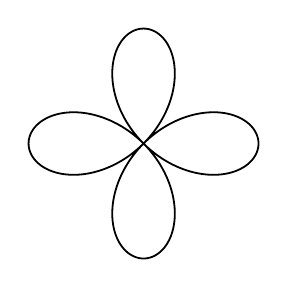
\begin{tikzpicture}[x=0.365cm,y=0.365cm]
  \polargrid
  \draw[line width=0.65pt,samples=361,smooth,domain=0:360] plot ({(4*cos(2*\x))*cos(\x)},{(4*cos(2*\x))*sin(\x)});
\end{tikzpicture}
&
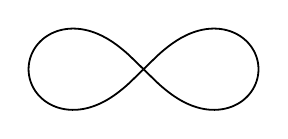
\begin{tikzpicture}[x=0.365cm,y=0.365cm]
  \polargrid
  \draw[line width=0.65pt,samples=101,smooth,domain=-45:45] plot ({(4*sqrt(cos(2*\x)))*cos(\x)},{(4*sqrt(cos(2*\x)))*sin(\x)});
  \draw[line width=0.65pt,samples=101,smooth,domain=135:225] plot ({(4*sqrt(cos(2*\x)))*cos(\x)},{(4*sqrt(cos(2*\x)))*sin(\x)});
\end{tikzpicture}
&

\begin{tikzpicture}[x=0.365cm,y=0.365cm]
  \polargrid
  \draw[line width=0.65pt,samples=361,smooth,domain=0:360] plot ({(4/(2-cos(\x)))*cos(\x)},{(4/(2-cos(\x)))*sin(\x)});
\end{tikzpicture}
\\[-0.2em]
\textup{(1)} & \textup{(2)} & \textup{(3)} & \textup{(4)}
\end{tabular}
\end{center}
\end{problem}

% 2021 Spring KAIST Calculus I Final, Problem 5
\begin{problem}[2021 Spring \KAIST{} Calculus I]
Let
\[
L_1:\ x=1+t,\ y=3-t,\ z=2t,
\qquad
L_2:\ x=0,\ y=-2s,\ z=5s.
\]
Find the minimum of $\|\overrightarrow{P_1P_2}\|$ for $P_1\in L_1$ and $P_2\in L_2$.
\end{problem}

% 2021 Spring KAIST Calculus I Final, Problem 7
\begin{problem}[2021 Spring \KAIST{} Calculus I]
Let $M_1$ be the plane in space given by
\[
2x-y-3z=2,
\]
and let $M_2$ be the plane perpendicular to $M_1$ through the points $P(1,-2,-4)$ and $Q(0,-1,-2)$.
\begin{problemsubparts}
\item Find parametric equations for the line $L$ of intersection of $M_1$ and $M_2$.
\item Find an equation for a plane $M$ parallel to $L$ that contains the line through the points $A(-2,-4,3)$ and $B(2,0,4)$. Find the distance between $L$ and $M$.
\end{problemsubparts}
\end{problem}

% 2021 Spring KAIST Calculus I Final, Problem 8
\begin{problem}[2021 Spring \KAIST{} Calculus I]
For the surface with equation
\[
(y-\sqrt{2z_0})^2-x^2=z,
\]
consider its curve cut $C$ by the plane $z=z_0>0$.
\begin{problemsubparts}
\item Identify the type of $C$ and find its eccentricity.
\item Find the foci and directrices of the curve cut on the plane $z=z_0$.
\item Find the polar equation $r=f(\theta)$ of the curve cut on the plane $z=z_0$.
\end{problemsubparts}
\end{problem}


% 2021 Fall POSTECH Calculus II Midterm, Problem 1
\begin{problem}[2021 Fall \POSTECH{} Calculus II]
Find an equation of the plane that passes through the line of intersection of the planes
\[
x+y=2
\qquad\text{and}\qquad
2x-y+3z=1
\]
and passes through the point $(1,2,1)$.
\end{problem}

% 2021 Fall POSTECH Calculus II Midterm, Problem 2
\begin{problem}[2021 Fall \POSTECH{} Calculus II]
Let $f(x,y)=|xy|$. Show that $f$ is differentiable at $(0,0)$.
\end{problem}

% 2021 Fall POSTECH Calculus II Midterm, Problem 3
\begin{problem}[2021 Fall \POSTECH{} Calculus II]
Let $F(x,y,z)$ be differentiable everywhere. Assume that
\[
F(1+t^2,2t,-1-t)=0
\]
for all $t$, and that $\nabla F(2,2,-3)=(a,b,c)$. Show that
\[
a+b=\frac{c}{2}.
\]
\end{problem}

% 2021 Fall POSTECH Calculus II Midterm, Problem 4
\begin{problem}[2021 Fall \POSTECH{} Calculus II]
A plane $P$ contains the points $(-3,0,0)$, $(0,-3,0)$, and $(0,0,-3)$. Find all points on
\[
z=x^2+y^2
\]
whose tangent plane does not intersect $P$.
\end{problem}

% 2021 Fall POSTECH Calculus II Midterm, Problem 5
\begin{problem}[2021 Fall \POSTECH{} Calculus II]
Find the absolute maximum and minimum values of
\[
f(x,y)=x^4+y^4-4xy+1
\]
on the region
\[
x^4+y^4\le 1.
\]
\end{problem}

% 2021 Fall POSTECH Calculus II Midterm, Problem 6
\begin{problem}[2021 Fall \POSTECH{} Calculus II]
Let $L_1$ and $L_2$ be lines in $\R^3$ parametrized by
\[
L_1(t)=(1+t,1-t,2t),
\qquad
L_2(s)=(-s,s,-s),
\]
respectively. Find the shortest distance between $L_1$ and $L_2$.
\end{problem}

% 2021 Fall POSTECH Calculus II Midterm, Problem 7
\begin{problem}[2021 Fall \POSTECH{} Calculus II]
Let $f(x,y)=|xy|$. Show that there is no open ball centered at $(0,0)$ in which $f_x$ and $f_y$ are defined and continuous.
\end{problem}

% 2021 Fall POSTECH Calculus II Midterm, Problem 8
\begin{problem}[2021 Fall \POSTECH{} Calculus II]
% The source is preserved exactly here: it uses (xy)^alpha rather than |xy|^alpha.
Let
\[
f(x,y)=
\begin{cases}
\displaystyle\frac{(xy)^\alpha}{x^2+y^2}, & (x,y)\ne(0,0),\\[0.55em]
0, & (x,y)=(0,0).
\end{cases}
\]
For which $\alpha>0$ is $f$ differentiable in $\R^2$?
\end{problem}

% 2021 Fall POSTECH Calculus II Midterm, Problem 9
\begin{problem}[2021 Fall \POSTECH{} Calculus II]
Let
\[
R=\left\{(x,y):0\le x\le\frac{\sqrt3}{2},\ 0\le y\le\frac{\sqrt3}{2},\ x^2+y^2\le1\right\}.
\]
Find the minimum and maximum of the linear function
\[
F(x,y)=-x+2y.
\]
Justify your answer.
\end{problem}

% 2021 Fall POSTECH Calculus II Midterm, Problem 10
\begin{problem}[2021 Fall \POSTECH{} Calculus II]
Show that
\[
f(x,y)=x^2-2xy^2-y^4
\]
has a saddle point at $(0,0)$.
\end{problem}


% 2021 Fall POSTECH Calculus II Final, Problem 1
\begin{problem}[2021 Fall \POSTECH{} Calculus II]
Show by giving a counterexample that the cross product is not associative; namely, find three vectors $\mathbf U,\mathbf V,\mathbf W\in\R^3$ such that
\[
(\mathbf U\times\mathbf V)\times\mathbf W
\ne
\mathbf U\times(\mathbf V\times\mathbf W).
\]
\end{problem}

% 2021 Fall POSTECH Calculus II Final, Problem 2
\begin{problem}[2021 Fall \POSTECH{} Calculus II]
Determine the maximum and minimum values of
\[
f(x,y)=xy\ln(1+x^2+y^2)
\]
in the region
\[
x^2+y^2\le1.
\]
\end{problem}

% 2021 Fall POSTECH Calculus II Final, Problem 3
\begin{problem}[2021 Fall \POSTECH{} Calculus II]
Evaluate
\[
I_x=\iiint_D x\,\dd V,
\]
where
\[
D=\left\{(x,y,z):1\le x^2+y^2+z^2\le4,\ x\ge0\right\}.
\]
\end{problem}

% 2021 Fall POSTECH Calculus II Final, Problem 4
\begin{problem}[2021 Fall \POSTECH{} Calculus II]
Evaluate the surface integral
\[
\iint_S \mathbf F\cdot\mathbf N\,\dd S
\]
representing the flux of the vector field
\[
\mathbf F(x,y,z)=(1+x,x+2y,-3x+z)
\]
across the hemisphere
\[
S=\left\{(x,y,z):x^2+y^2+z^2=1,\ x\ge0\right\}
\]
in the direction of the unit normal vector field whose first component is positive.
\end{problem}

% 2021 Fall POSTECH Calculus II Final, Problem 5
\begin{problem}[2021 Fall \POSTECH{} Calculus II]
Let $S\subseteq\R^3$ be the surface defined by
\[
y=x^2+z^2,
\qquad x^2+z^2\le1.
\]

\Needspace{12\baselineskip}
\begin{center}
\begin{tikzpicture}[x=1cm,y=1cm,line cap=round,line join=round]
  \draw[-{Stealth[length=2.0mm]},line width=0.45pt] (0,0) -- (4.15,0) node[right] {$y$};
  \draw[-{Stealth[length=2.0mm]},line width=0.45pt] (0,0) -- (-1.05,-0.72) node[below left] {$x$};
  \draw[-{Stealth[length=2.0mm]},line width=0.45pt] (0,0) -- (0,1.72) node[above] {$z$};
  \draw[line width=0.75pt,samples=60,smooth,domain=0:1] plot ({3.15*\x},{1.18*sqrt(\x)});
  \draw[line width=0.75pt,samples=60,smooth,domain=0:1] plot ({3.15*\x},{-1.18*sqrt(\x)});
  \foreach \t in {0.2,0.4,0.6,0.8,1.0}{%
    \pgfmathsetmacro{\rx}{0.38*sqrt(\t)}%
    \pgfmathsetmacro{\rz}{1.18*sqrt(\t)}%
    \draw[gray!65,line width=0.35pt] ({3.15*\t},0) ellipse [x radius=\rx cm,y radius=\rz cm];
  }
  \draw[line width=0.8pt] (3.15,0) ellipse [x radius=0.38cm,y radius=1.18cm];
  \node at (2.05,0.78) {$S$};
\end{tikzpicture}
\end{center}

Let
\[
\mathbf F(x,y,z)=(y,z,x).
\]
Find the inward flux of $\nabla\times\mathbf F$ across $S$ in the direction of the unit normal vector field whose second component is positive.
\end{problem}

% 2021 Fall POSTECH Calculus II Final, Problem 6
\begin{problem}[2021 Fall \POSTECH{} Calculus II]
Let
\[
f(x,y)=|(x-1)(y-1)|.
\]
Show that there is no open ball centered at $(1,1)$ in which $f_x$ and $f_y$ are defined and continuous.
\end{problem}

% 2021 Fall POSTECH Calculus II Final, Problem 7
\begin{problem}[2021 Fall \POSTECH{} Calculus II]
Find the volume of the solid $E$ bounded by both the sphere
\[
x^2+y^2+z^2=2z
\]
and the sphere
\[
x^2+y^2+z^2=\frac14.
\]
\end{problem}

% 2021 Fall POSTECH Calculus II Final, Problem 8
\begin{problem}[2021 Fall \POSTECH{} Calculus II]
An object moves from the origin to a point that lies on the surface
\[
\frac{x^2}{a^2}+\frac{y^2}{b^2}+\frac{z^2}{c^2}=1
\]
along a smooth curve $C$ under the force field
\[
\mathbf F(x,y,z)=(yz,zx,xy).
\]
Find the maximum possible value of the work integral
\[
\int_C\mathbf F\cdot\dd\mathbf r.
\]
\end{problem}

% 2021 Fall POSTECH Calculus II Final, Problem 9
\begin{problem}[2021 Fall \POSTECH{} Calculus II]
Let $C$ be the triangle shown below, oriented counterclockwise.

\Needspace{11\baselineskip}
\begin{center}
\begin{tikzpicture}[scale=1.25,line cap=round,line join=round]
  \draw[-{Stealth[length=2mm]},line width=0.45pt] (-0.25,0) -- (1.55,0) node[right] {$x$};
  \draw[-{Stealth[length=2mm]},line width=0.45pt] (0,-0.22) -- (0,1.55) node[above] {$y$};
  \draw[line width=0.8pt] (0,0) -- (1,0) -- (0,1) -- cycle;
  \draw[-{Stealth[length=2mm]},line width=0.55pt] (0.30,0) -- (0.68,0);
  \draw[-{Stealth[length=2mm]},line width=0.55pt] (0.78,0.22) -- (0.54,0.46);
  \draw[-{Stealth[length=2mm]},line width=0.55pt] (0,0.70) -- (0,0.32);
  \node[below] at (1,0) {$1$};
  \node[left] at (0,1) {$1$};
  \node at (0.56,0.56) {$C$};
\end{tikzpicture}
\end{center}

Evaluate
\[
\oint_C x^2\,\dd y.
\]
\end{problem}

% 2021 Fall POSTECH Calculus II Final, Problem 10
\begin{problem}[2021 Fall \POSTECH{} Calculus II]
Let $S\subseteq\R^3$ be a surface with a parametrization $\boldsymbol{\alpha}\colon\mathcal R\to S$ defined by
\[
\boldsymbol{\alpha}(u,v)
=uv\mathbf i+\frac{u}{v}\mathbf j+\frac{v}{u}\mathbf k.
\]
Find an equation for the tangent plane to $S$ at $\boldsymbol{\alpha}(1,1)$.
\end{problem}

% 2021 Fall KAIST Calculus I Final, Problem 1
\begin{problem}[2021 Fall \KAIST{} Calculus I]
Mark True or False for each of the following statements. You do not need to justify your answers.
\begin{problemchoices}
\item If a series $\displaystyle\sum_{n=0}^{\infty}a_nx^n$ converges on $[-1,1]$, then the series $\displaystyle\sum_{n=1}^{\infty}na_nx^{n-1}$ converges on $(-1,1)$.
\item If $\mathbf a,\mathbf b,\mathbf c$ are three-dimensional vectors, then
\[
\mathbf a\times(\mathbf b\times\mathbf c)=(\mathbf a\times\mathbf b)\times\mathbf c.
\]
\item If $\mathbf a,\mathbf b,\mathbf c$ are nonzero three-dimensional vectors and $(\mathbf a\times\mathbf b)\cdot\mathbf c=0$, then $\mathbf a,\mathbf b,\mathbf c$ are in the same plane.
\item Assume $f$ is infinitely differentiable at $0$ (i.e., $f^{(n)}(0)$ exists for all $n=1,2,3,\ldots$). Then there exists $\varepsilon>0$ such that
\[
f(x)=\sum_{n=0}^{\infty}\frac{f^{(n)}(0)}{n!}x^n
\]
for all $-\varepsilon<x<\varepsilon$.
\item Let $A(x)=\displaystyle\sum_n a_nx^n$ and $B(x)=\displaystyle\sum_n b_nx^n$ be power series with radii of convergence $R_1$ and $R_2$, respectively. Then $A(x)B(x)$ is again a power series with radius of convergence $\min\{R_1,R_2\}$.
\end{problemchoices}
\end{problem}

% 2021 Fall KAIST Calculus I Final, Problem 2
\begin{problem}[2021 Fall \KAIST{} Calculus I]
Let $\{\mathbf{x}_n\}$ be a sequence of vectors, where
\[
\mathbf{x}_n=(x_n^{(1)},x_n^{(2)},x_n^{(3)}).
\]
Let $\mathbf{x}$ be a vector. Prove or disprove:
\begin{problemsubparts}
\item $\|\mathbf{x}_n-\mathbf{x}\|\to0$ if $\displaystyle\sum_{k=1}^{n}\|\mathbf{x}_k-\mathbf{x}\|\le1$ for all $n$.
\item $\|\mathbf{x}_n-\mathbf{x}\|\to0$ if
\[
\lim_{n\to\infty}\frac{\|\mathbf{x}_{n+1}-\mathbf{x}\|}{\|\mathbf{x}_n-\mathbf{x}\|}=\rho<1.
\]
\end{problemsubparts}
\end{problem}

% 2021 Fall KAIST Calculus I Final, Problem 5
\begin{problem}[2021 Fall \KAIST{} Calculus I]
How many domains are separately enclosed by the following polar equations?
\begin{problemchoices}
\item $r=4\cos(2\theta)$
\item $\displaystyle r=\frac{4}{2-\cos\theta}$
\item $r=2(1+\cos\theta)$
\end{problemchoices}
\end{problem}

% 2021 Fall KAIST Calculus I Final, Problem 6
\begin{problem}[2021 Fall \KAIST{} Calculus I]
Consider the curve
\[
r=\cos3\theta,
\qquad -\frac{\pi}{6}\le\theta\le\frac{\pi}{6}.
\]
\begin{problemsubparts}
\item Find the slopes of the curve at the origin.
\item Find the length of the curve, using the fact that
\[
\int_0^{\pi/3}\sqrt{1+8\sin^2 3\theta}\,\dd\theta\approx2.23.
\]
\item Find the area enclosed by the curve.
\end{problemsubparts}
\end{problem}

% 2021 Fall KAIST Calculus I Final, Problem 7
\begin{problem}[2021 Fall \KAIST{} Calculus I]
Your eye is at $(4,0,0)$. You are looking at a triangular plate whose vertices are at $(1,0,1)$, $(1,1,0)$, and $(-2,2,2)$. The line segment from $(1,0,0)$ to $(0,2,2)$ passes through the plate. What portion of the line segment is hidden from your view by the plate?
\end{problem}

% 2021 Fall KAIST Calculus I Final, Problem 8
\begin{problem}[2021 Fall \KAIST{} Calculus I]
Let
\[
L_1:\ x=1+t,\ y=3-t,\ z=2t,
\qquad
L_2:\ x=0,\ y=-2s,\ z=5s.
\]
Find the minimum of $\|\overrightarrow{P_1P_2}\|$ for $P_1\in L_1$ and $P_2\in L_2$.
\end{problem}


% 2022 Spring KAIST Calculus II Midterm, Problem 1
\begin{problem}[2022 Spring \KAIST{} Calculus II]
Answer the following True/False questions. You do not need to justify your answers.
\begin{problemsubparts}
\item Let $\mathbf r(t)$ be a parametrization of the movement of a particle along a smooth curve in space. If its speed $|\mathbf r'(t)|$ is constant, then its principal unit normal vector $\mathbf N$ and its acceleration $\mathbf r''(t)$ are parallel.
\item Let $f(x,y)$ be a function of two variables. If the directional derivative $D_{\mathbf u}f$ exists for each direction $\mathbf u$, then $f$ is continuous at $(0,0)$.
\item A smooth space curve $\mathbf r(t)$ with zero torsion is necessarily contained in a plane.
\item Let $\mathbf r(t)$ be a smooth curve on the sphere
\[
x^2+y^2+z^2=R^2,
\qquad R>0.
\]
Then its curvature is always at least $1/R$, i.e., $\kappa\ge 1/R$.
\item Consider the surface $z=z(x,y)$ given by
\[
x^2+\frac{(y-z)^2}{z^2}=1,
\qquad z>0.
\]
The level curve has an increasing curvature at the origin $(0,0)$ as the level increases.
\end{problemsubparts}
\end{problem}

% 2022 Spring KAIST Calculus II Midterm, Problem 2
\begin{problem}[2022 Spring \KAIST{} Calculus II]
Let $C$ be a smooth curve in space parametrized by $\mathbf r(t)$.
\begin{problemsubparts}
\item Express $\mathbf r'$ and $\mathbf r''$ in the TNB frame.
\item Using (a), deduce the following expression for the curvature:
\[
\kappa(t)=
\frac{|x'y''-x''y'|}{\bigl((x')^2+(y')^2\bigr)^{3/2}}
\]
for $\mathbf r(t)=(x(t),y(t))$.
\end{problemsubparts}
\end{problem}

% 2022 Spring KAIST Calculus II Midterm, Problem 3
\begin{problem}[2022 Spring \KAIST{} Calculus II]
Consider the ellipse
\[
\frac{x^2}{9}+\frac{y^2}{4}=1.
\]
\begin{problemsubparts}
\item Find the point(s) where the curvature is minimum.
\item Find the equation of the circle of curvature at the point(s) where the curvature is minimum.
\end{problemsubparts}
\end{problem}

% 2022 Spring KAIST Calculus II Midterm, Problem 4
\begin{problem}[2022 Spring \KAIST{} Calculus II]
Let
\[
f(x,y)=
\begin{cases}
\displaystyle\frac{4x^2y^2}{x^4-2xy^2+y^3}, & (x,y)\ne(0,0),\\[0.6em]
0, & (x,y)=(0,0).
\end{cases}
\]
\begin{problemsubparts}
\item Calculate $f_x(0,0)$ and $f_y(0,0)$.
\item Calculate the directional derivative $D_{\mathbf u}f(0,0)$, where $\mathbf u$ is the unit vector in the direction of $(1,1)$.
\end{problemsubparts}
\end{problem}

% 2022 Spring KAIST Calculus II Midterm, Problem 5
\begin{problem}[2022 Spring \KAIST{} Calculus II]
Let $C$ be the circular helix in $\R^3$ given by
\[
\mathbf r(t)=(3\cos t,3\sin t,4t)
\]
from the point $P_0=(3,0,0)$ to the point $P_1=(3,0,8\pi)$.
\begin{problemsubparts}
\item Find the arc length of $C$ from $P_0$ to $P_1$, and reparametrize $C$ by the arc length function $s(t)$.
\item Find the unit tangent vector $\mathbf T$ of $C$ at the point $(-3,0,4\pi)$.
\item Calculate the curvature $\kappa$ of $C$, and find the principal unit normal vector $\mathbf N$ of $C$ at the point $(-3,0,4\pi)$.
\end{problemsubparts}
\end{problem}

% 2022 Spring KAIST Calculus II Midterm, Problem 6
\begin{problem}[2022 Spring \KAIST{} Calculus II]
Let
\[
f(x,y)=
\begin{cases}
\displaystyle\frac{\sin\!\bigl(x^3(y^3+\pi)\bigr)}{x^2+y^2}, & (x,y)\ne(0,0),\\[0.6em]
0, & (x,y)=(0,0).
\end{cases}
\]
\textit{Hint.} $\displaystyle\lim_{t\to0}\frac{\sin t}{t}=1$.
\begin{problemsubparts}
\item Show that
\[
\lim_{(x,y)\to(0,0)}\frac{x^3(y^3+\pi)}{x^2+y^2}=0.
\]
\item Prove that $f$ is continuous at $(0,0)$.
\item Calculate $f_x(0,0)$ and $f_y(0,0)$.
\end{problemsubparts}
\end{problem}

% 2022 Spring KAIST Calculus II Midterm, Problem 7
\begin{problem}[2022 Spring \KAIST{} Calculus II]
Consider the function
\[
f(x,y)=4x^2y+x^2y^2+8xy^2+2xy^3+1.
\]
Find all critical points and classify them.
\end{problem}

% 2022 Spring KAIST Calculus II Midterm, Problem 8
\begin{problem}[2022 Spring \KAIST{} Calculus II]
Consider the surface $C$ given by
\[
z=x^2+y^2
\]
and the point $P=(3,3,1)$ in space. Find the equation of the sphere with center $P$ which is tangent to $C$.
\end{problem}

% 2022 Spring KAIST Calculus II Midterm, Problem 9
\begin{problem}[2022 Spring \KAIST{} Calculus II]
Find the extreme values of the function
\[
f(x,y,z)=xy+z^2
\]
on the circle in which the plane $x=y$ intersects the sphere
\[
x^2+y^2+z^2=4.
\]
\end{problem}

% 2022 Spring KAIST Calculus II Midterm, Problem 10
\begin{problem}[2022 Spring \KAIST{} Calculus II]
Consider the function
\[
f(x,y)=\cos x\cos y.
\]
\begin{problemsubparts}
\item Use Taylor's formula to find a quadratic approximation near the origin $(0,0)$.
\item Estimate the error in the approximation if $|x|\le0.1$ and $|y|\le0.1$. You do not need to compute exact values; simply find a numerical expression.
\end{problemsubparts}
\end{problem}

% 2022 Spring KAIST Calculus II Midterm, Problem 11
\begin{problem}[2022 Spring \KAIST{} Calculus II]
Consider the function $f(x,y)$ given by
\[
f(x,y)=
\begin{cases}
x^m y^n, & \begin{aligned}&\text{if either $x$ is rational and $y$ is irrational,}\\[-0.15em]&\text{or $x$ is irrational and $y$ is rational,}\end{aligned}\\[0.8em]
0, & \text{otherwise},
\end{cases}
\]
for some nonnegative integers $m$ and $n$. Let $0^0=1$.
\begin{problemsubparts}
\item Find all nonnegative integers $m$ and $n$ such that $f$ is continuous at $(0,0)$.
\item Find all nonnegative integers $m$ and $n$ such that $f$ is differentiable at $(0,0)$.
\end{problemsubparts}
\end{problem}

% 2022 Spring KAIST Calculus II Final, Problem 1
\begin{problem}[2022 Spring \KAIST{} Calculus II]
Answer the following True/False questions. You do not need to justify your answers.
\begin{problemsubparts}
\item Let $\mathbf F=(M,N,P)$ be a vector field on $\R^3$ whose components $M$, $N$, and $P$ have continuous second partial derivatives. Then
\[
\nabla\cdot(\nabla\times\mathbf F)=0.
\]
\item For a function $f\colon[0,1]\times[0,1]\to\R$, suppose that the iterated integrals
\[
\int_0^1\int_0^1 f(x,y)\,\dd x\,\dd y
\qquad\text{and}\qquad
\int_0^1\int_0^1 f(x,y)\,\dd y\,\dd x
\]
exist and are equal. Then $f$ is integrable.
\item Let $\mathbf F=(M,N,P)$ be a vector field on an open connected domain $D\subseteq\R^3$ whose components $M$, $N$, and $P$ have continuous first partial derivatives and satisfy
\[
\frac{\partial N}{\partial x}=\frac{\partial M}{\partial y},
\qquad
\frac{\partial P}{\partial y}=\frac{\partial N}{\partial z},
\qquad
\frac{\partial M}{\partial z}=\frac{\partial P}{\partial x}.
\]
Then $\mathbf F$ is conservative on $D$.
\item There is a piecewise smooth, simple loop in $\R^2$ whose principal unit normal vector $\mathbf N$ and outward unit normal vector $\mathbf n$ are coincident.
\item Let $C$ be a clockwise-oriented, piecewise smooth, simple loop in $\R^2$ whose curvature never vanishes. Let $\mathbf N$ be the principal unit normal vector of $C$. Then, for any vector field $\mathbf F$ on $\R^2$ whose components have continuous first partial derivatives,
\[
\int_C \mathbf F\cdot\mathbf N\,\dd s
+
\iint_D \nabla\cdot\mathbf F\,\dd A
=0,
\]
where $D$ is the region surrounded by $C$.
\end{problemsubparts}
\end{problem}

% 2022 Spring KAIST Calculus II Final, Problem 2
\begin{problem}[2022 Spring \KAIST{} Calculus II]
Evaluate the integral
\[
\int_0^1\int_x^1\int_{\sqrt y}^{1}
\frac{e^{z^3}}{z^2}\,\dd z\,\dd y\,\dd x.
\]
\end{problem}

% 2022 Spring KAIST Calculus II Final, Problem 3
\begin{problem}[2022 Spring \KAIST{} Calculus II]
Consider the vector field
\[
\mathbf F(x,y)=
\left(
-\frac{y}{x^2+y^2},
\frac{x}{x^2+y^2}
\right)
\]
on $\R^2\setminus\{(0,0)\}$. Calculate the line integral
\[
\oint_C\mathbf F\cdot\dd\mathbf r
\]
over each of the following curves, oriented counterclockwise.
\begin{problemsubparts}
\item $C_1\colon (x-2)^2+(y+1)^2=4$.
\item $C_2\colon x^2+y^2=9$.
\item $C_3\colon r=9+4\sin 3\theta$, where $(x,y)=(r\cos\theta,r\sin\theta)$.
\end{problemsubparts}
\end{problem}

% 2022 Spring KAIST Calculus II Final, Problem 4
\begin{problem}[2022 Spring \KAIST{} Calculus II]
\begin{problemsubparts}
\item Calculate the divergence of the vector field
\[
\mathbf F(x,y)=
\bigl(xy e^{x^2+y^2},xy e^{x^2+y^2}\bigr)
\]
on the plane $\R^2$.
\item Calculate the double integral
\[
\iint_R (x+y)(1+2xy)e^{x^2+y^2}\,\dd A,
\]
where
\[
R=[0,1]\times[0,1]
=\{(x,y)\in\R^2:0\le x,y\le1\}.
\]
\end{problemsubparts}
\end{problem}

% 2022 Spring KAIST Calculus II Final, Problem 5
\begin{problem}[2022 Spring \KAIST{} Calculus II]
Consider the parallelogram $R$ given by the lines
\[
L_1\colon y=\frac{x}{2},
\qquad
L_2\colon y=-\frac{5x}{3},
\qquad
L_3\colon y=\frac{x+13}{2},
\qquad
L_4\colon y=\frac{-5x+13}{3}.
\]
Calculate the area $A(R)$ of the parallelogram $R$ in the following steps.
\begin{problemsubparts}
\item Find a linear transformation $\boldsymbol{\Phi}\colon\R^2\to\R^2$ sending the unit square $[0,1]\times[0,1]$ to the parallelogram $R$.

\textit{Hint.} If $\boldsymbol{\Phi}$ is linear, then
\[
\boldsymbol{\Phi}(u,v)
=\boldsymbol{\Phi}(1,0)u+\boldsymbol{\Phi}(0,1)v
\]
for all $(u,v)\in\R^2$.
\item Calculate $A(R)$ using the transformation $\boldsymbol{\Phi}$.
\end{problemsubparts}
\end{problem}

% 2022 Spring KAIST Calculus II Final, Problem 6
\begin{problem}[2022 Spring \KAIST{} Calculus II]
Use cylindrical coordinates to find the volume of the solid in $\R^3$ enclosed by the cone
\[
z=\sqrt{x^2+y^2},
\]
the cylinder
\[
x^2+(y-1)^2=1,
\]
and the $xy$-plane.

\textit{Hint.} $\sin^3\theta=(1-\cos^2\theta)\sin\theta$.
\end{problem}

% 2022 Spring KAIST Calculus II Final, Problem 7
\begin{problem}[2022 Spring \KAIST{} Calculus II]
Let $\mathbf h(x,y)$ be a smooth parametrization on a region $H$ for a surface $S$ in $\R^3$. Suppose that there is a transformation
\[
\mathbf F\colon R\to H,
\qquad
(u,v)\mapsto(x(u,v),y(u,v)),
\]
such that $\mathbf F$ is one-to-one on the interior of the region $R$, its components have continuous first partial derivatives, and $\mathbf r=\mathbf h\circ\mathbf F$ is a smooth parametrization on $R$ for $S$. Show that
\[
\iint_H |\mathbf h_x\times\mathbf h_y|\,\dd x\,\dd y
=
\iint_R |\mathbf r_u\times\mathbf r_v|\,\dd u\,\dd v
=A(S).
\tag{\(\star\)}
\]
where $A(S)$ is the area of $S$, in the following steps.
\begin{problemsubparts}
\item Show that
\[
\mathbf r_u\times\mathbf r_v
=
(\mathbf h_x\times\mathbf h_y)
\frac{\partial(x,y)}{\partial(u,v)},
\]
where $\partial(x,y)/\partial(u,v)$ is the Jacobian of the transformation $\mathbf F$.
\item Use (a) to deduce $(\star)$.
\end{problemsubparts}
\end{problem}

% 2022 Spring KAIST Calculus II Final, Problem 8
\begin{problem}[2022 Spring \KAIST{} Calculus II]
Let $D$ be the solid region with ellipsoidal boundary $\partial D$:
\[
x^2+y^2+\frac{z^2}{4}=9,
\]
which is oriented with the unit normal vector pointing outward.
\begin{problemsubparts}
\item Calculate the volume of $D$.
\item Let $\mathbf F$ be the vector field on $\R^3$ given by
\[
\mathbf F(x,y,z)=
\left(
x^2\sqrt{y^2+z^2},
-y^2\sqrt{x^2+z^2},
z^2\sqrt{x^2+y^2}
\right).
\]
Calculate the surface integral
\[
\iint_{\partial D}\mathbf F\cdot\mathbf n\,\dd S,
\]
where $\mathbf n$ is the outward unit normal vector.
\end{problemsubparts}
\end{problem}

% 2022 Spring KAIST Calculus II Final, Problem 9
\begin{problem}[2022 Spring \KAIST{} Calculus II]
Let $S$ be the surface given by
\[
x^2+y^2+(z-3)^2=5^2,
\qquad
z\ge0,
\]
and let $\mathbf n$ be the unit normal vector on $S$ pointing outward from the origin. Calculate the surface integral
\[
\iint_S (\nabla\times\mathbf F)\cdot\mathbf n\,\dd S
\]
for the vector field
\[
\mathbf F(x,y,z)=
\left(
\frac{x}{1+x^4}-\sin(e^{-y}),
\frac{y}{1+y^6}+\sin(e^x),
e^{-x^2-y^2-z^2}
\right).
\]
\textit{Hint.} For $R\colon x^2+y^2\le4$,
\[
\iint_R e^x\cos(e^x)\,\dd A
=
\iint_R e^{-y}\cos(e^{-y})\,\dd A.
\]
\end{problem}

% 2022 Spring KAIST Calculus II Final, Problem 10
\begin{problem}[2022 Spring \KAIST{} Calculus II]
Consider the function
\[
f\colon[0,1]\times[0,1]\subseteq\R^2\to\R
\]
defined by
\[
f(x,y)=
\begin{cases}
\sin\bigl(2\pi(x+y)\bigr), & \text{if $y$ is rational},\\
-\sin\bigl(2\pi(x+y)\bigr), & \text{if $y$ is irrational}.
\end{cases}
\]
\begin{problemsubparts}
\item Show that the iterated integral
\[
\int_0^1\int_0^1 f(x,y)\,\dd x\,\dd y
\]
exists, and evaluate it.
\item Show that $f$ is not integrable over $[0,1]\times[0,1]$.
\end{problemsubparts}
\end{problem}

% 2022 Fall POSTECH Calculus II Midterm, Problem 1
\begin{problem}[2022 Fall \POSTECH{} Calculus II]
Let $\ell$ be a line in $\R^4$ passing through $(0,1,-1,3)$ and parallel to $(1,0,3,-1)$. If $P=(6,5,4,2)$ is a point not on $\ell$, find the distance between $\ell$ and $P$.
\end{problem}

% 2022 Fall POSTECH Calculus II Midterm, Problem 2
\begin{problem}[2022 Fall \POSTECH{} Calculus II]
Let $f(x,y)=x^3+3y$.
\begin{problemsubparts}
\item Find an equation of the plane tangent to the graph of $f$ at $(2,4)$.
\item Find the linear approximation of $f(x,y)$ near $(2,4)$, and use it to estimate $f(2.01,4.03)$.
\end{problemsubparts}
\end{problem}

% 2022 Fall POSTECH Calculus II Midterm, Problem 3
\begin{problem}[2022 Fall \POSTECH{} Calculus II]
The Laplace operator $\Delta$ is defined by
\[
\Delta=\partial_{xx}+\partial_{yy}.
\]
Compute
\[
\Delta\ln\!\left(\sqrt{x^2+y^2}\right),
\qquad (x,y)\ne(0,0).
\]
\end{problem}

% 2022 Fall POSTECH Calculus II Midterm, Problem 4
\begin{problem}[2022 Fall \POSTECH{} Calculus II]
\begin{problemsubparts}
\item Let $f\colon\R^n\to\R$ be linear. Show that there exist numbers $C_j$, $j=1,\ldots,n$, such that
\[
f(\mathbf x)=\sum_{j=1}^n C_jx_j,
\qquad \mathbf x=(x_1,\ldots,x_n).
\]
\item Show that
\[
f(\mathbf x)=\sum_{j=1}^n C_jx_j
\]
is differentiable on $\R^n$. Find $\nabla f$.
\end{problemsubparts}
\end{problem}

% 2022 Fall POSTECH Calculus II Midterm, Problem 5
\begin{problem}[2022 Fall \POSTECH{} Calculus II]
Determine whether each of the following functions is continuous, and prove your answers.
\begin{problemsubparts}
\item
\[
f(x,y)=
\begin{cases}
\displaystyle\frac{xy}{x^2+y^2}, & (x,y)\ne(0,0),\\[0.55em]
0, & (x,y)=(0,0).
\end{cases}
\]
\item
\[
f(x,y)=
\begin{cases}
\displaystyle\frac{x^2y}{x^2+y^2}, & (x,y)\ne(0,0),\\[0.55em]
0, & (x,y)=(0,0).
\end{cases}
\]
\end{problemsubparts}
\noindent\textit{Hint.} Use polar coordinates.
\end{problem}

% 2022 Fall POSTECH Calculus II Midterm, Problem 6
\begin{problem}[2022 Fall \POSTECH{} Calculus II]
Let
\[
f(x,y)=\frac1{1-xy}.
\]
Find the second-order Taylor approximation to $f$ at $(0,0)$.
\end{problem}

% 2022 Fall POSTECH Calculus II Midterm, Problem 7
\begin{problem}[2022 Fall \POSTECH{} Calculus II]
A line $L_1$ in $\R^3$ is given by
\[
x=t+1,
\qquad y=t+2,
\qquad z=t+3,
\]
and a line $L_2$ in $\R^3$ is given by
\[
x=1-s,
\qquad y=1+s,
\qquad z=2s.
\]
Find a point $P$ on $L_1$ and a point $Q$ on $L_2$ such that the square of the distance between $P$ and $Q$ is a local minimum with respect to $t$ and $s$.
\end{problem}

% 2022 Fall POSTECH Calculus II Midterm, Problem 8
\begin{problem}[2022 Fall \POSTECH{} Calculus II]
Let
\[
f(x,y)=x^2+3y^2,
\qquad
g(x,y)=x^4+2y^2.
\]
\begin{problemsubparts}
\item Show that $f$ and $g$ attain their strict local minimum at the origin $(0,0)$.
\item Show that $\Hess f(0,0)$ is positive definite but $\Hess g(0,0)$ is not positive definite.
\end{problemsubparts}
\end{problem}

\Needspace{22\baselineskip}
% 2022 Fall POSTECH Calculus II Midterm, Problem 9
\begin{problem}[2022 Fall \POSTECH{} Calculus II]
Let $C$ be the curve in $\R^2$ defined by
\[
x^3+y^2=1.
\]
The minimum distance from a point on $C$ to the point $(-1,0)$ occurs at $(a,\pm b)\in C$, where $b>1$.

\Needspace{14\baselineskip}
\begin{center}
\begin{tikzpicture}[scale=1.02,line cap=round,line join=round]
  \draw[-{Stealth[length=2mm]},line width=0.45pt] (-1.45,0) -- (1.45,0) node[right] {$x$};
  \draw[-{Stealth[length=2mm]},line width=0.45pt] (0,-1.75) -- (0,1.75) node[above] {$y$};
  \draw[line width=0.8pt] plot[smooth] coordinates {(-1.1598,-1.6000) (-1.1276,-1.5600) (-1.0943,-1.5200) (-1.0598,-1.4800) (-1.0240,-1.4400) (-0.9865,-1.4000) (-0.9471,-1.3600) (-0.9055,-1.3200) (-0.8611,-1.2800) (-0.8131,-1.2400) (-0.7606,-1.2000) (-0.7018,-1.1600) (-0.6336,-1.1200) (-0.5500,-1.0800) (-0.4337,-1.0400) (0.0000,-1.0000) (0.4280,-0.9600) (0.5355,-0.9200) (0.6088,-0.8800) (0.6652,-0.8400) (0.7114,-0.8000) (0.7503,-0.7600) (0.7838,-0.7200) (0.8131,-0.6800) (0.8389,-0.6400) (0.8618,-0.6000) (0.8821,-0.5600) (0.9002,-0.5200) (0.9164,-0.4800) (0.9308,-0.4400) (0.9435,-0.4000) (0.9548,-0.3600) (0.9646,-0.3200) (0.9732,-0.2800) (0.9804,-0.2400) (0.9865,-0.2000) (0.9914,-0.1600) (0.9952,-0.1200) (0.9979,-0.0800) (0.9995,-0.0400) (1.0000,0.0000) (0.9995,0.0400) (0.9979,0.0800) (0.9952,0.1200) (0.9914,0.1600) (0.9865,0.2000) (0.9804,0.2400) (0.9732,0.2800) (0.9646,0.3200) (0.9548,0.3600) (0.9435,0.4000) (0.9308,0.4400) (0.9164,0.4800) (0.9002,0.5200) (0.8821,0.5600) (0.8618,0.6000) (0.8389,0.6400) (0.8131,0.6800) (0.7838,0.7200) (0.7503,0.7600) (0.7114,0.8000) (0.6652,0.8400) (0.6088,0.8800) (0.5355,0.9200) (0.4280,0.9600) (0.0000,1.0000) (-0.4337,1.0400) (-0.5500,1.0800) (-0.6336,1.1200) (-0.7018,1.1600) (-0.7606,1.2000) (-0.8131,1.2400) (-0.8611,1.2800) (-0.9055,1.3200) (-0.9471,1.3600) (-0.9865,1.4000) (-1.0240,1.4400) (-1.0598,1.4800) (-1.0943,1.5200) (-1.1276,1.5600) (-1.1598,1.6000)};
  \fill (-0.5486,1.0794) circle (1.35pt);
  \fill (-0.5486,-1.0794) circle (1.35pt);
  \node[above left] at (-0.5486,1.0794) {$(a,b)$};
  \node[below left] at (-0.5486,-1.0794) {$(a,-b)$};
  \node[above left] at (-0.88,1.55) {$C$};
  \draw[line width=0.4pt] (-1,0.055)--(-1,-0.055) node[below] {$-1$};
  \draw[line width=0.4pt] (0.055,1)--(-0.055,1) node[left] {$1$};
  \draw[line width=0.4pt] (0.055,-1)--(-0.055,-1) node[left] {$-1$};
\end{tikzpicture}
\end{center}

Check the conditions for using the Lagrange multiplier method. Find $a$ using the Lagrange multiplier method.
\end{problem}

% 2022 Fall POSTECH Calculus II Midterm, Problem 10
\begin{problem}[2022 Fall \POSTECH{} Calculus II]
Consider the function
\[
f(x,y,z)=x^4+y^4+z^4-4xyz.
\]
\begin{problemsubparts}
\item Find all $P\in\R^3$ such that $\nabla f(P)=\mathbf0$.
\item Show that at each local extremum except the origin, $f$ has a local minimum.
\item Show that $f(0,0,0)$ is not a local extremum.
\end{problemsubparts}
\end{problem}


% 2022 Fall POSTECH Calculus II Final, Problem 1
\begin{problem}[2022 Fall \POSTECH{} Calculus II]
Write a Riemann sum for
\[
\iint_{[0,1]\times[0,1]}x^2y^3\,\dd A
\]
using points at the upper-right corner of each $\frac14$-square.
\end{problem}

% 2022 Fall POSTECH Calculus II Final, Problem 2
\begin{problem}[2022 Fall \POSTECH{} Calculus II]
Let $D$ be the parallelogram in $\R^2$ bounded by the lines
\[
y=-x+5,
\qquad y=-x+2,
\qquad y=2x-1,
\qquad y=2x-4.
\]
Compute
\[
\iint_D y^2\,\dd A.
\]
\end{problem}

\Needspace{18\baselineskip}
% 2022 Fall POSTECH Calculus II Final, Problem 3
\begin{problem}[2022 Fall \POSTECH{} Calculus II]
An orange is cut into three slices with equal width.

\Needspace{14\baselineskip}
\begin{center}
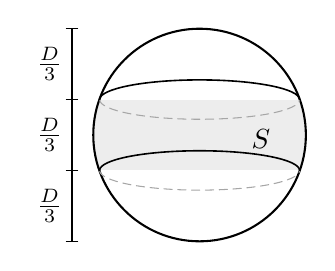
\begin{tikzpicture}[scale=1.0,line cap=round,line join=round]
  \begin{scope}
    \clip (0,0) circle (1.35);
    \fill[gray!14] (-1.45,-0.45) rectangle (1.45,0.45);
  \end{scope}
  \draw[line width=0.75pt] (0,0) circle (1.35);
  \draw[densely dashed,gray!70,line width=0.38pt] (-1.27,0.45) arc[start angle=180,end angle=360,x radius=1.27,y radius=0.25];
  \draw[line width=0.58pt] (1.27,0.45) arc[start angle=0,end angle=180,x radius=1.27,y radius=0.25];
  \draw[densely dashed,gray!70,line width=0.38pt] (-1.27,-0.45) arc[start angle=180,end angle=360,x radius=1.27,y radius=0.25];
  \draw[line width=0.58pt] (1.27,-0.45) arc[start angle=0,end angle=180,x radius=1.27,y radius=0.25];
  \node at (0.78,-0.05) {$S$};
  \draw[line width=0.38pt] (-1.62,-1.35)--(-1.62,1.35);
  \foreach \yy in {-1.35,-0.45,0.45,1.35}{\draw[line width=0.38pt] (-1.69,\yy)--(-1.55,\yy);}
  \node[left] at (-1.62,0.90) {$\frac D3$};
  \node[left] at (-1.62,0.00) {$\frac D3$};
  \node[left] at (-1.62,-0.90) {$\frac D3$};
\end{tikzpicture}
\end{center}

Assume that the surface of the orange is a sphere with diameter $D$. Find the area of the peel from the middle slice (the area of $S$ in the figure) by evaluating a surface integral explicitly.
\end{problem}

% 2022 Fall POSTECH Calculus II Final, Problem 4
\begin{problem}[2022 Fall \POSTECH{} Calculus II]
Find
\[
\oint_C\mathbf F\cdot\mathbf T\,\dd s,
\]
where
\[
\mathbf F(x,y)=\left(-\frac{y}{x^2+y^2},\frac{x}{x^2+y^2}\right),
\]
and $C$ is a loop that contains the origin in its interior and is traversed counterclockwise.
\end{problem}

% 2022 Fall POSTECH Calculus II Final, Problem 5
\begin{problem}[2022 Fall \POSTECH{} Calculus II]
Let
\[
\mathbf F(x,y,z)=(x^2+y,\sin y,z).
\]
\begin{problemsubparts}
\item Verify that $\mathbf F$ is not conservative.
\item Verify that
\[
\mathbf G(x,y,z)=(x^2,\sin y,z)
\]
is conservative.
\item Find the integral of $\mathbf F$ along the curve $C=C_1\cup C_2\cup C_3$ shown below, using part (b).
\end{problemsubparts}

\Needspace{18\baselineskip}
\begin{center}
\begin{tikzpicture}[scale=1.05,line cap=round,line join=round]
  \coordinate (O) at (0,0);
  \coordinate (A) at (-1.30,-0.50); % (2,0,0)
  \coordinate (B) at (-1.30,0.35);  % (2,0,1)
  \coordinate (C) at (0.30,0.15);   % (2,2,1)
  \coordinate (D) at (1.60,2.35);   % (0,2,3)
  \coordinate (Y2) at (1.60,-0.20);
  \coordinate (Z3) at (0,2.55);
  \draw[-{Stealth[length=2mm]},line width=0.42pt] (O)--(-1.85,-0.72) node[below left] {$x$};
  \draw[-{Stealth[length=2mm]},line width=0.42pt] (O)--(2.35,-0.28) node[right] {$y$};
  \draw[-{Stealth[length=2mm]},line width=0.42pt] (O)--(0,2.75) node[above] {$z$};
  \draw[densely dashed,gray!60,line width=0.35pt] (A)--(O);
  \draw[densely dashed,gray!60,line width=0.35pt] (C)--(0.30,-0.62)--(1.60,-0.20);
  \draw[densely dashed,gray!60,line width=0.35pt] (D)--(1.60,-0.20);
  \draw[line width=0.82pt,-{Stealth[length=2mm]}] (A)--(B);
  \draw[line width=0.82pt,-{Stealth[length=2mm]}] (B)--(C);
  \draw[line width=0.82pt,-{Stealth[length=2mm]}] (C)--(D);
  \foreach \P in {A,B,C,D}{\fill (\P) circle (1.25pt);}
  \node[below] at (A) {$(2,0,0)$};
  \node[left] at (B) {$(2,0,1)$};
  \node[below right] at (C) {$(2,2,1)$};
  \node[right] at (D) {$(0,2,3)$};
  \node[left] at (-1.40,-0.05) {$C_1$};
  \node[above] at (-0.50,0.34) {$C_2$};
  \node[left] at (0.85,1.28) {$C_3$};
\end{tikzpicture}
\end{center}
\end{problem}

% 2022 Fall POSTECH Calculus II Final, Problem 6
\begin{problem}[2022 Fall \POSTECH{} Calculus II]
For each of the following statements, answer True or False. Here $C$ is a smooth curve in $\R^2$, $-C$ is $C$ traversed in the opposite direction, and $\mathbf T_C$ and $\mathbf T_{-C}$ are the unit tangent vectors to $C$ and $-C$, respectively. The vector field $\mathbf F$ is continuously differentiable on $\R^2$.
\begin{problemchoices}
\item $\displaystyle\int_C f\,\dd s=-\int_{-C}f\,\dd s$, where $f\colon\R^2\to\R$ is continuous.
\item $\displaystyle\int_C\mathbf F\cdot\mathbf T_C\,\dd s=-\int_{-C}\mathbf F\cdot\mathbf T_{-C}\,\dd s$.
\item $\displaystyle\int_C\mathbf F\cdot\mathbf N\,\dd s=-\int_{-C}\mathbf F\cdot\mathbf N\,\dd s$ with the same unit normal vector $\mathbf N$.
\item $\mathbf F$ is conservative if and only if $\operatorname{curl}\mathbf F=0$.
\item
\[
\int_{h(a)}^{h(b)}g(x)\,\dd x
=
\int_a^b g(h(t))|h'(t)|\,\dd t,
\]
where $g\colon\R\to\R$ is continuous and $h\colon[a,b]\to\R$ is $C^1$.
\end{problemchoices}
\end{problem}

% 2022 Fall POSTECH Calculus II Final, Problem 7
\begin{problem}[2022 Fall \POSTECH{} Calculus II]
\begin{problemsubparts}
\item State Stokes' theorem, including all conditions.
\item Let
\[
D=\left\{(x,y,z)\in\R^3:x^2+y^2+z^2=5^2,\ y\le-1\right\}.
\]
Find the area of $D$. Verify Stokes' theorem for the vector field
\[
\mathbf F(x,y,z)=(-z,-4,x).
\]
\end{problemsubparts}
\end{problem}

% 2022 Fall POSTECH Calculus II Final, Problem 8
\begin{problem}[2022 Fall \POSTECH{} Calculus II]
Let $\mathbf F(x,y,z)=(x,y,z)$, and let $S\subseteq\R^3$ be the surface defined by
\[
y+2z^2=2,
\qquad 0\le x\le1,
\qquad 0\le z\le1.
\]
\Needspace{17\baselineskip}
\begin{center}
\begin{tikzpicture}[x=1cm,y=1cm,line cap=round,line join=round]
  % Axes under the surface.
  \draw[-{Stealth[length=2mm]},line width=0.42pt] (0,0) -- (-1.38,-0.64) node[below left] {$x$};
  \draw[-{Stealth[length=2mm]},line width=0.42pt] (0,0) -- (2.85,0) node[right] {$y$};
  \draw[-{Stealth[length=2mm]},line width=0.42pt] (0,0) -- (0,1.75) node[above] {$z$};
  % Surface y+2z^2=2, 0<=x<=1, 0<=z<=1.
  \path[fill=gray!12]
    plot[samples=50,smooth,domain=0:1] ({1.2*(2-2*\x*\x)},{1.15*\x})
    -- plot[samples=50,smooth,domain=1:0] ({1.2*(2-2*\x*\x)-0.95},{1.15*\x-0.44}) -- cycle;
  \draw[line width=0.72pt]
    plot[samples=50,smooth,domain=0:1] ({1.2*(2-2*\x*\x)},{1.15*\x});
  \draw[line width=0.72pt]
    plot[samples=50,smooth,domain=0:1] ({1.2*(2-2*\x*\x)-0.95},{1.15*\x-0.44});
  \draw[line width=0.72pt] (2.40,0) -- (1.45,-0.44);
  \draw[line width=0.72pt] (0,1.15) -- (-0.95,0.71);
  \foreach \zz in {0.2,0.4,0.6,0.8}{
    \pgfmathsetmacro{\yy}{2-2*\zz*\zz}
    \draw[gray!62,line width=0.32pt] ({1.2*\yy},{1.15*\zz}) -- ({1.2*\yy-0.95},{1.15*\zz-0.44});
  }
  \foreach \xx in {0.25,0.5,0.75}{
    \draw[gray!62,line width=0.32pt]
      plot[samples=38,smooth,domain=0:1] ({1.2*(2-2*\x*\x)-0.95*\xx},{1.15*\x-0.44*\xx});
  }
  % Outward-normal cues, matching the information in the source figure.
  \foreach \zz/\xx in {0.23/0.18,0.50/0.48,0.73/0.76}{
    \pgfmathsetmacro{\yy}{2-2*\zz*\zz}
    \pgfmathsetmacro{\px}{1.2*\yy-0.95*\xx}
    \pgfmathsetmacro{\py}{1.15*\zz-0.44*\xx}
    \draw[-{Stealth[length=1.9mm]},line width=0.48pt] (\px,\py) -- ++(0.25,0.34);
  }
  \node at (0.86,0.54) {$S$};
  \node[below right] at (1.56,-0.27) {$\partial S$};
  \node[below] at (-0.95,-0.44) {$1$};
  \node[below] at (2.40,0) {$2$};
  \node[left] at (0,1.15) {$1$};
\end{tikzpicture}
\end{center}
\begin{problemsubparts}
\item Find the outward flux of $\mathbf F$ across $S$ by evaluating a surface integral.
\item Find the counterclockwise circulation of $\mathbf F$ around $\partial S$.
\end{problemsubparts}
\end{problem}

% 2022 Fall POSTECH Calculus II Final, Problem 9
\begin{problem}[2022 Fall \POSTECH{} Calculus II]
Let $\mathbf F=(xy,z,2y)$ be a vector field in $\R^3$, and let $C$ be a curve of intersection of the plane
\[
x+z=5
\]
and the cylinder
\[
x^2+y^2=9.
\]
Orient $C$ so that its projection onto the $xy$-plane is oriented clockwise. Find
\[
\int_C\mathbf F\cdot\mathbf T\,\dd s.
\]
\end{problem}

% 2022 Fall POSTECH Calculus II Final, Problem 10
\begin{problem}[2022 Fall \POSTECH{} Calculus II]
Use each of the following theorems to show that, for a regular set $D\subseteq\R^2$ with boundary oriented counterclockwise,
\[
\area(D)=-\int_{\partial D}y\,\dd x.
\]
\begin{problemsubparts}
\item Use the Divergence theorem.
\item Use Green's theorem.
\end{problemsubparts}
\end{problem}

% 2022 Fall POSTECH Calculus II Final, Problem 11
\begin{problem}[2022 Fall \POSTECH{} Calculus II]
Let
\[
\mathbf F(x,y,z)=(y+z,z+x,x+y)
\]
be a vector field in $\R^3$, and let $C$ be a piecewise smooth curve from the origin to any point on the unit sphere
\[
x^2+y^2+z^2=1.
\]
Find the maximum of
\[
\int_C\mathbf F\cdot\mathbf T\,\dd s.
\]
\end{problem}

% 2022 Fall POSTECH Calculus II Final, Problem 12
\begin{problem}[2022 Fall \POSTECH{} Calculus II]
Let $\mathbf F(x,y,z)=(x,y,z)$, and let $S\subseteq\R^3$ be the surface defined by
\[
y+2z^2=2,
\qquad 0\le x\le1,
\qquad 0\le z\le1.
\]
\Needspace{17\baselineskip}
\begin{center}
\begin{tikzpicture}[x=1cm,y=1cm,line cap=round,line join=round]
  % Axes under the surface.
  \draw[-{Stealth[length=2mm]},line width=0.42pt] (0,0) -- (-1.38,-0.64) node[below left] {$x$};
  \draw[-{Stealth[length=2mm]},line width=0.42pt] (0,0) -- (2.85,0) node[right] {$y$};
  \draw[-{Stealth[length=2mm]},line width=0.42pt] (0,0) -- (0,1.75) node[above] {$z$};
  % Surface y+2z^2=2, 0<=x<=1, 0<=z<=1.
  \path[fill=gray!12]
    plot[samples=50,smooth,domain=0:1] ({1.2*(2-2*\x*\x)},{1.15*\x})
    -- plot[samples=50,smooth,domain=1:0] ({1.2*(2-2*\x*\x)-0.95},{1.15*\x-0.44}) -- cycle;
  \draw[line width=0.72pt]
    plot[samples=50,smooth,domain=0:1] ({1.2*(2-2*\x*\x)},{1.15*\x});
  \draw[line width=0.72pt]
    plot[samples=50,smooth,domain=0:1] ({1.2*(2-2*\x*\x)-0.95},{1.15*\x-0.44});
  \draw[line width=0.72pt] (2.40,0) -- (1.45,-0.44);
  \draw[line width=0.72pt] (0,1.15) -- (-0.95,0.71);
  \foreach \zz in {0.2,0.4,0.6,0.8}{
    \pgfmathsetmacro{\yy}{2-2*\zz*\zz}
    \draw[gray!62,line width=0.32pt] ({1.2*\yy},{1.15*\zz}) -- ({1.2*\yy-0.95},{1.15*\zz-0.44});
  }
  \foreach \xx in {0.25,0.5,0.75}{
    \draw[gray!62,line width=0.32pt]
      plot[samples=38,smooth,domain=0:1] ({1.2*(2-2*\x*\x)-0.95*\xx},{1.15*\x-0.44*\xx});
  }
  % Outward-normal cues, matching the information in the source figure.
  \foreach \zz/\xx in {0.23/0.18,0.50/0.48,0.73/0.76}{
    \pgfmathsetmacro{\yy}{2-2*\zz*\zz}
    \pgfmathsetmacro{\px}{1.2*\yy-0.95*\xx}
    \pgfmathsetmacro{\py}{1.15*\zz-0.44*\xx}
    \draw[-{Stealth[length=1.9mm]},line width=0.48pt] (\px,\py) -- ++(0.25,0.34);
  }
  \node at (0.86,0.54) {$S$};
  \node[below right] at (1.56,-0.27) {$\partial S$};
  \node[below] at (-0.95,-0.44) {$1$};
  \node[below] at (2.40,0) {$2$};
  \node[left] at (0,1.15) {$1$};
\end{tikzpicture}
\end{center}
Using the Divergence theorem, find the outward flux of $\mathbf F$ across $S$.

\noindent\textit{Hint.} Consider a three-dimensional solid whose boundary contains $S$.
\end{problem}

% 2022 Fall POSTECH Calculus II Final, Problem 13
\begin{problem}[2022 Fall \POSTECH{} Calculus II]
\begin{problemsubparts}
\item Show that
\[
\nabla\cdot(v\nabla u)=v\Delta u+\nabla v\cdot\nabla u
\]
for all twice differentiable functions $u$ and $v$ on a regular set $D\subset\R^3$.
\item Derive the following equality for a twice differentiable function $u$ on $D$:
\[
\iiint_D\left(u\Delta u+\|\nabla u\|^2\right)\,\dd V
=
\iint_{\partial D}u\nabla u\cdot\mathbf N\,\dd S,
\]
where $\mathbf N$ is the unit outward normal vector on the boundary $\partial D$.
\item Let $u$ be a twice differentiable function satisfying
\[
\Delta u=u\quad\text{in }D,
\qquad
u=0\quad\text{on }\partial D.
\]
Show that $u\equiv0$.
\end{problemsubparts}
\end{problem}

% 2022 Fall KAIST Calculus II Midterm, Problem 1
\begin{problem}[2022 Fall \KAIST{} Calculus II]
The K9 Thunder is a Korean 155 mm self-propelled howitzer (cannon). Its maximum range is $18\,\mathrm{km}$. It depends on the type of cannonball fired.
\begin{problemsubparts}
\item Use the equations for projectile motion studied in class to find the initial speed of the cannonball. Take $g=9.8\,\mathrm{m/s^2}$.
\item How many seconds does it take to hit the target at the maximum range?
\end{problemsubparts}
\end{problem}

% 2022 Fall KAIST Calculus II Midterm, Problem 2
\begin{problem}[2022 Fall \KAIST{} Calculus II]
Let $C$ be a curve parametrized by
\[
\mathbf r(t)=(\cos t,\sin t,\sin t\cos t).
\]
\begin{problemsubparts}
\item Find the curvature $\kappa$ of $C$ at the point
\[
\mathbf r\!\left(\frac{\pi}{4}\right)
=\left(\frac{1}{\sqrt2},\frac{1}{\sqrt2},\frac12\right).
\]
\item Find the torsion $\tau$ of $C$ at the point
\[
\mathbf r\!\left(\frac{\pi}{3}\right)
=\left(\frac12,\frac{\sqrt3}{2},\frac{\sqrt3}{4}\right).
\]
\end{problemsubparts}
\end{problem}

% 2022 Fall KAIST Calculus II Midterm, Problem 3
\begin{problem}[2022 Fall \KAIST{} Calculus II]
Let $C$ be the curve
\[
\mathbf r(t)
=(\cos t-2\sin t+1,\sin t+2\cos t,2t).
\]
\begin{problemsubparts}
\item Find the TNB frame vectors $\mathbf T$, $\mathbf N$, and $\mathbf B$ at $\mathbf r(\pi)$.
\item Find the equation of the osculating plane (the tangent plane orthogonal to $\mathbf B$) of $C$ at $\mathbf r(\pi)$.
\end{problemsubparts}
\end{problem}

% 2022 Fall KAIST Calculus II Midterm, Problem 4
\begin{problem}[2022 Fall \KAIST{} Calculus II]
The gravitational force between the Earth and a satellite is given by
\[
\mathbf F
=-\frac{GmM}{|\mathbf r|^2}\frac{\mathbf r}{|\mathbf r|},
\]
where $M$ is the mass of the Earth, $m$ is the mass of the satellite, $G$ is the universal gravitational constant, and $\mathbf r$ is the position vector of the satellite when the Earth is at the origin.
\begin{problemsubparts}
\item Suppose that the satellite orbits the Earth along a circular orbit. Let $r(t)=|\mathbf r(t)|$ be the radius and $\theta(t)$ be the angle at time $t$. Find the formula for the circular motion of the satellite.
\item Find the escape energy for the satellite, or equivalently the minimum work required to send the satellite to infinity from the Earth's surface. Let $R$ be the radius of the Earth.
\end{problemsubparts}
\end{problem}

% 2022 Fall KAIST Calculus II Midterm, Problem 5
\begin{problem}[2022 Fall \KAIST{} Calculus II]
Determine, with justification, whether each of the following limits exists.
\begin{problemsubparts}
\item
\[
\lim_{(x,y)\to(1,1)}\frac{xy^2-1}{y-1}.
\]
\item
\[
\lim_{(x,y)\to(1,0)}\frac{xe^y-1}{xe^y-1+y}.
\]
\end{problemsubparts}
\end{problem}

% 2022 Fall KAIST Calculus II Midterm, Problem 6
\begin{problem}[2022 Fall \KAIST{} Calculus II]
Let
\[
f(x,y)=
\begin{cases}
\displaystyle\frac{xy(x^2-y^2)}{x^2+y^2}, & (x,y)\ne(0,0),\\[0.6em]
0, & (x,y)=(0,0).
\end{cases}
\]
\begin{problemsubparts}
\item Find $\dfrac{\partial f}{\partial y}(x,0)$ for all $x$ and $\dfrac{\partial f}{\partial x}(0,y)$ for all $y$.
\item Find
\[
\frac{\partial^2 f}{\partial x\,\partial y}(0,0)
\qquad\text{and}\qquad
\frac{\partial^2 f}{\partial y\,\partial x}(0,0).
\]
\end{problemsubparts}
\end{problem}

% 2022 Fall KAIST Calculus II Midterm, Problem 7
\begin{problem}[2022 Fall \KAIST{} Calculus II]
Define $f\colon\R^2\to\R$ by
\[
f(0,0)=0,
\qquad
f(x,y)=\frac{x(x+y)^2}{y^4+x^2}
\quad\text{if }(x,y)\ne(0,0).
\]
Let $S$ be the set of all directions (unit vectors) $\mathbf u=x\mathbf i+y\mathbf j$, let $X\subset S$ be the collection of directions for which the directional derivative $D_{\mathbf u}f(0,0)$ exists, and define
\[
g(x,y)=D_{\mathbf u}f(0,0).
\]
\begin{problemsubparts}
\item Find $X$ and $g(x,y)$. Decide whether $g$ is continuous on $X$.
\item Find the absolute and local extreme values of $g$, if they exist.
\end{problemsubparts}
\end{problem}

% 2022 Fall KAIST Calculus II Midterm, Problem 8
\begin{problem}[2022 Fall \KAIST{} Calculus II]
\begin{problemsubparts}
\item Let
\[
f(x,y)=x^2+2kxy+3y^2.
\]
For what values of $k$ does $f$ have a local minimum at $(0,0)$? For what values of $k$ does $f$ have a saddle point at $(0,0)$?
\item Let
\[
w=x^2-y^2+4z+t,
\qquad
x+2z+t=25,
\qquad
x+z+y=0.
\]
Compute $\partial w/\partial x$ when $x$ and $y$ are considered independent variables.
\end{problemsubparts}
\end{problem}

% 2022 Fall KAIST Calculus II Midterm, Problem 9
\begin{problem}[2022 Fall \KAIST{} Calculus II]
Let
\[
f(x,y)=\sin x\sin y.
\]
\begin{problemsubparts}
\item Use Taylor's formula to find a cubic approximation of $f$ at $(0,0)$, up to third-order terms.
\item Find an error estimate for the cubic approximation when $|x|<0.1$ and $|y|<0.1$, using fourth-order terms.
\end{problemsubparts}
\end{problem}

% 2022 Fall KAIST Calculus II Midterm, Problem 10
\begin{problem}[2022 Fall \KAIST{} Calculus II]
Find the minimum distance from the intersection $S=S_1\cap S_2$ to the origin, where
\[
S_1=\{(x,y,z):x^2+2y^2-z^2-1=0\},
\]
\[
S_2=\{(x,y,z):z^2-2z+2-2x^2-y^2=0\}.
\]
\end{problem}

% 2022 Fall KAIST Calculus II Final, Problem 1
\begin{problem}[2022 Fall \KAIST{} Calculus II]
In this problem, we will prove that the ``inverse'' Fubini theorem does not work for Riemann integrals and discontinuous functions. Recall that a binary-rational number is a number of the form $n/2^k$, where $k$ and $n$ are integers. Every binary-rational number except $0$ can be written in this form with an odd $n$ in a unique way. Let
\[
f(x,y)=1
\]
if $x=n/2^k$ and $y=m/2^k$, where $n$ and $m$ are odd integers and $k$ is any integer; note that the same $k$ is used in both expressions. Let $f(x,y)=0$ otherwise.
\begin{problemsubparts}
\item For a fixed $y=y_0\in[0,1]$, what are the values of $x\in[0,1]$ such that $f(x,y_0)=1$? How many such values are there? Your answer will depend on $y_0$.

Does the integral
\[
\int_0^1 f(x,y_0)\,\dd x
\]
exist? If so, what is its value?

Does the repeated integral
\[
\int_0^1\int_0^1 f(x,y)\,\dd x\,\dd y
\]
exist?
\item For a rectangle $R=[a,b]\times[c,d]$, where
\[
0\le a<b\le1,
\qquad
0\le c<d\le1,
\]
what are the minimum and maximum values of $f$ on $R$?

Does the double integral
\[
\iint_{[0,1]\times[0,1]} f(x,y)\,\dd x\,\dd y
\]
exist?
\end{problemsubparts}
\end{problem}

% 2022 Fall KAIST Calculus II Final, Problem 2
\begin{problem}[2022 Fall \KAIST{} Calculus II]
Let
\[
D=\{(x,y)\in\R^2:x^2+y^2\le2x\text{ and }x^2+y^2\le2\sqrt3\,y\}
\]
be the region in the $xy$-plane.
\begin{problemsubparts}
\item Split
\[
\iint_D f(x,y)\,\dd A
\]
into a sum of two iterated integrals in polar form.
\item Find the area of $D$.
\end{problemsubparts}
\end{problem}

% 2022 Fall KAIST Calculus II Final, Problem 3
\begin{problem}[2022 Fall \KAIST{} Calculus II]
Let $R$ be a region in the first octant $(x,y,z>0)$ in $\R^3$ satisfying
\[
x+y^2+4z^2\le4.
\]
\begin{problemsubparts}
\item Describe the triple integral
\[
\iiint_R f(x,y,z)\,\dd V
\]
as an iterated integral (i) in the order $\dd x\,\dd y\,\dd z$ and (ii) in the order $\dd y\,\dd z\,\dd x$.
\item Evaluate
\[
\iiint_R yz\,\dd V.
\]
\end{problemsubparts}
\end{problem}

% 2022 Fall KAIST Calculus II Final, Problem 4
\begin{problem}[2022 Fall \KAIST{} Calculus II]
Let $R$ be a region in the first quadrant of the $xy$-plane bounded by
\[
xy=4,
\qquad
xy=16,
\qquad
y=x,
\qquad
y=9x.
\]
\begin{problemsubparts}
\item Use the transformation
\[
x=\frac{u}{v},
\qquad
y=uv,
\qquad u>0,
\qquad v>0,
\]
and find a region $G$ in the $uv$-plane and a function $f(u,v)$ such that
\[
\iint_R\left(\sqrt{\frac{y}{x}}+\sqrt{xy}\right)\,\dd x\,\dd y
=
\iint_G f(u,v)\,\dd u\,\dd v.
\]
\item Evaluate the above integral.
\end{problemsubparts}
\end{problem}

% 2022 Fall KAIST Calculus II Final, Problem 5
\begin{problem}[2022 Fall \KAIST{} Calculus II]
Let
\[
\boldsymbol{\Phi}(u,v)
=u\sin v\,\mathbf i-v\,\mathbf j+u\cos v\,\mathbf k,
\qquad
0\le u\le1,
\qquad
0\le v\le\pi.
\]
\begin{problemsubparts}
\item Describe the smooth component curves of the boundary curve of the surface defined by $\boldsymbol{\Phi}$. Identify the one, say $C$, with maximum arc length.
\item Let
\[
f(x,y,z)=z^4e^x-3(e^x+3y)xz^2.
\]
Find the point on $C$ that divides $C$ into two curves $C_1$ and $C_2$ of equal arc length. Evaluate the line integrals of $f$ along the curves $C_1$ and $C_2$.
\end{problemsubparts}
\end{problem}

% 2022 Fall KAIST Calculus II Final, Problem 6
\begin{problem}[2022 Fall \KAIST{} Calculus II]
Let $\mathbf F=M\mathbf i+N\mathbf j$, and let $C$ be a simple, closed curve enclosing a region $D$ in the plane.
\begin{problemsubparts}
\item State the two versions of Green's Theorem and derive one version from the other.
\item Let
\[
M=\frac{x^4}{4},
\qquad
N=x^3y,
\qquad
C=\left\{(x,y)\in\R^2:\frac{x^4}{a^4}+\frac{y^2}{b^2}=1\right\}.
\]
Find the outward flux
\[
\int_C\mathbf F\cdot\mathbf n\,\dd s
=
\int_C M\,\dd y-N\,\dd x.
\]
\end{problemsubparts}
\end{problem}

% 2022 Fall KAIST Calculus II Final, Problem 7
\begin{problem}[2022 Fall \KAIST{} Calculus II]
Let
\[
\mathbf F=x\mathbf i+y\mathbf j+z\mathbf k
\]
and let $S$ be the ellipsoid
\[
\frac{x^2}{a^2}+\frac{y^2}{b^2}+\frac{z^2}{c^2}=1,
\qquad a,b,c>0.
\]
\begin{problemsubparts}
\item Use spherical coordinates $(\phi,\theta)$ and find a parametrization of $S$ in the form
\[
\mathbf r(\phi,\theta)
=(x(\phi,\theta),y(\phi,\theta),z(\phi,\theta)),
\]
and compute $\mathbf r_\phi\times\mathbf r_\theta$.
\item Compute $\mathbf n\,\dd S$ and the outward flux
\[
\iint_S\mathbf F\cdot\mathbf n\,\dd S.
\]
\end{problemsubparts}
\end{problem}

% 2022 Fall KAIST Calculus II Final, Problem 8
\begin{problem}[2022 Fall \KAIST{} Calculus II]
Let $\mathbf F=M\mathbf i+N\mathbf j+P\mathbf k$ be continuously differentiable, let
\[
S=\{(x,y,z)\in\R^3:x^2+y^2+z^2=1\}
\]
be the unit sphere, let
\[
S_1=\{(x,y,z)\in S:z\ge0\},
\qquad
S_2=\{(x,y,z)\in S:z\le0\}
\]
be the upper and lower hemispheres, and let
\[
B=\{(x,y,z):x^2+y^2+z^2\le1\}
\]
be the unit ball.
\begin{problemsubparts}
\item Use the fact that $S=S_1\cup S_2$ and Stokes' Theorem to show that
\[
\iint_S(\nabla\times\mathbf F)\cdot\mathbf n\,\dd S=0.
\]
\item Use the Divergence Theorem to show that
\[
\iiint_B\nabla\cdot(\nabla\times\mathbf F)\,\dd V=0.
\]
\end{problemsubparts}
\end{problem}

% 2022 Fall KAIST Calculus II Final, Problem 9
\begin{problem}[2022 Fall \KAIST{} Calculus II]
Let $(x,y)\in\R^2$ be fixed, let $\varepsilon>0$ be small, let
\[
A_\varepsilon=[x,x+\varepsilon]\times[y,y+\varepsilon]
\]
be a small square cell, and let $C_\varepsilon=\partial A_\varepsilon$ be its boundary. Let $\mathbf F=M\mathbf i+N\mathbf j$ be twice differentiable and suppose that
\[
|M_{xx}|,|M_{xy}|,|M_{yy}|,|N_{xx}|,|N_{xy}|,|N_{yy}|\le K_0,
\]
i.e., all second-order partial derivatives of $M$ and $N$ are bounded by $K_0$. Note that the area of $A_\varepsilon$ is $\Delta(A_\varepsilon)=\varepsilon^2$. Use Taylor's formula and show that
\[
\left|
\int_{C_\varepsilon}\mathbf F\cdot\mathbf n\,\dd s
-
\bigl(M_x(x,y)+N_y(x,y)\bigr)\varepsilon^2
\right|
\le4K_0\varepsilon^3.
\]
\end{problem}

% 2022 Fall KAIST Calculus II Final, Problem 10
\begin{problem}[2022 Fall \KAIST{} Calculus II]
Let $D$ be a right cylinder, perpendicular to the $xy$-plane, whose base is the region between the circles
\[
r=\cos\theta
\qquad\text{and}\qquad
r=2\cos\theta,
\]
and whose top lies in the plane
\[
z=4-x-y.
\]
Find the volume of $D$.
\end{problem}

% 2023 Fall POSTECH Calculus II Midterm, Problem 1
\begin{problem}[2023 Fall \POSTECH{} Calculus II]
Find an equation for the plane tangent to
\[
x-3y^2+z^2=7
\]
at $(1,1,3)$.
\end{problem}

% 2023 Fall POSTECH Calculus II Midterm, Problem 2
\begin{problem}[2023 Fall \POSTECH{} Calculus II]
Let $L$ be the line containing $(1,2,1,1)$ and $(1,0,2,2)$ in $\R^4$. Let $P$ be the hyperplane defined by
\[
x+y+z+w=1
\]
in $\R^4$.
\begin{problemsubparts}
\item Do $L$ and $P$ intersect each other?
\item If the answer is yes, find the intersection point. Otherwise, find the distance between $L$ and $P$.
\end{problemsubparts}
\end{problem}

% 2023 Fall POSTECH Calculus II Midterm, Problem 3
\begin{problem}[2023 Fall \POSTECH{} Calculus II]
Let $f\colon\R^2\to\R$ be defined by
\[
f(x,y)=|x^3+y^3|.
\]
\begin{problemsubparts}
\item Find $\nabla f(0,0)$.
\item Is $f$ differentiable at $(0,0)$? Why or why not? Justify your answer.
\end{problemsubparts}
\end{problem}

% 2023 Fall POSTECH Calculus II Midterm, Problem 4
\begin{problem}[2023 Fall \POSTECH{} Calculus II]
Let $u\colon\R^2\to\R$ be a $C^2$ function, and define
\[
v(r,\theta)\coloneqq u(r\cos\theta,r\sin\theta).
\]
Show that
\[
u_{xx}+u_{yy}
=
v_{rr}+\frac1r v_r+\frac1{r^2}v_{\theta\theta}.
\]
\end{problem}

% 2023 Fall POSTECH Calculus II Midterm, Problem 5
\begin{problem}[2023 Fall \POSTECH{} Calculus II]
Suppose the electric potential at $(x,y)$ is given by
\[
\ln\!\left(\sqrt{x^2+y^2}\right).
\]
\begin{problemsubparts}
\item Find the rate of change of the potential at $(3,4)$ toward the origin.
\item Find the rate of change of the potential at $(3,4)$ in a direction perpendicular to the direction given above. You may choose either of the two possible directions.
\end{problemsubparts}
\end{problem}

% 2023 Fall POSTECH Calculus II Midterm, Problem 6
\begin{problem}[2023 Fall \POSTECH{} Calculus II]
Suppose there is a function $\mathbf F\colon\R^4\to\R^2$ with component functions $\mathbf F=(f_1,f_2)$ defined by
\[
\begin{aligned}
f_1(x,y,z,w)
&=e^{x+2y-z+w}-(2x^2-y^2+z^2-3w^2),\\
f_2(x,y,z,w)
&=\ln(1+x^2+y^2+z^2+w^2)+(3x+4y-5z+w).
\end{aligned}
\]
Let $P=(0,0,0,0)\in\R^4$.
\begin{problemsubparts}
\item Show that there is a differentiable function $\mathbf G\colon\R^2\to\R^2$ defined on a small open set $U$ around $(0,0)$ satisfying $\mathbf G(0,0)=(0,0)$ and
\[
\mathbf F(P)=\mathbf F\bigl(x,y,\mathbf G(x,y)\bigr)
\]
for $(x,y)\in U$.
\item Using the linear approximation of $\mathbf G$, find an approximate solution $(z,w)$ of the nonlinear system
\[
\begin{aligned}
1&=e^{0.1+2(0.1)-z+w}-\bigl(2(0.1)^2-(0.1)^2+z^2-3w^2\bigr),\\
0&=\ln\bigl(1+(0.1)^2+(0.1)^2+z^2+w^2\bigr)
   +\bigl(3(0.1)+4(0.1)-5z+w\bigr).
\end{aligned}
\]
\end{problemsubparts}
\end{problem}

% 2023 Fall POSTECH Calculus II Midterm, Problem 7
\begin{problem}[2023 Fall \POSTECH{} Calculus II]
Find the shortest distance from $(0,0,3)$ to the surface
\[
z=x^2-y^2.
\]
\end{problem}

% 2023 Fall POSTECH Calculus II Midterm, Problem 8
\begin{problem}[2023 Fall \POSTECH{} Calculus II]
Find the local maximum or minimum value of the function
\[
x^3+y^3+z^3-3xy-3yz-3zx
\]
defined on the domain
\[
\{(x,y,z):x>0,\ y>0,\ z>0\}.
\]
\end{problem}

% 2023 Fall POSTECH Calculus II Final, Problem 1
\begin{problem}[2023 Fall \POSTECH{} Calculus II]
Show that the function
\[
f(x,y)=x+y
\]
subject to the constraint
\[
x^3+x+y^3+y=1
\]
has at most one local extremum.
\end{problem}

% 2023 Fall POSTECH Calculus II Final, Problem 2
\begin{problem}[2023 Fall \POSTECH{} Calculus II]
Let $D\subseteq\R^2$ be the domain given by
\[
\frac{(x-1)^2}{4}+\frac{(y-3)^2}{9}\le1.
\]
Find
\[
\iint_D(x+y)\,\dd A.
\]
\end{problem}

% 2023 Fall POSTECH Calculus II Final, Problem 3
\begin{problem}[2023 Fall \POSTECH{} Calculus II]
A solid hemisphere of radius $R$ is split into two pieces with equal thickness. Use spherical coordinates to find the ratio of the volumes of the two pieces. Your answer should be a number between $0$ and $1$.

\Needspace{15\baselineskip}
\begin{center}
\begin{tikzpicture}[x=1cm,y=1cm,line cap=round,line join=round]
  % Hemisphere outline and base.
  \draw[line width=0.72pt] (-2.15,0) .. controls (-2.05,1.75) and (-1.08,2.55) .. (0,2.62)
    .. controls (1.08,2.55) and (2.05,1.75) .. (2.15,0);
  \draw[line width=0.72pt] (-2.15,0) arc[start angle=180,end angle=360,x radius=2.15,y radius=0.46];
  \draw[dashed,gray!68,line width=0.42pt] (2.15,0) arc[start angle=0,end angle=180,x radius=2.15,y radius=0.46];

  % Midplane z=R/2: back half dashed, front half solid.
  \draw[dashed,gray!68,line width=0.42pt] (1.82,1.31) arc[start angle=0,end angle=180,x radius=1.82,y radius=0.35];
  \draw[line width=0.65pt] (-1.82,1.31) arc[start angle=180,end angle=360,x radius=1.82,y radius=0.35];

  % Equal-thickness guides and labels.
  \draw[dashed,gray!58,line width=0.36pt] (-2.88,0) -- (-2.18,0);
  \draw[dashed,gray!58,line width=0.36pt] (-2.88,1.31) -- (-1.84,1.31);
  \draw[dashed,gray!58,line width=0.36pt] (-2.88,2.62) -- (0,2.62);
  \draw[{Stealth[length=1.6mm]}-{Stealth[length=1.6mm]},line width=0.42pt] (-2.58,0.08) -- (-2.58,1.23);
  \draw[{Stealth[length=1.6mm]}-{Stealth[length=1.6mm]},line width=0.42pt] (-2.58,1.39) -- (-2.58,2.54);
  \node[fill=white,inner sep=1.3pt] at (-2.58,0.655) {$\dfrac R2$};
  \node[fill=white,inner sep=1.3pt] at (-2.58,1.965) {$\dfrac R2$};

  % Radius cue on the base disk.
  \draw[-{Stealth[length=1.8mm]},line width=0.45pt] (0,-0.08) -- (1.72,-0.08);
  \node[fill=white,inner sep=1pt,above] at (0.90,-0.08) {$R$};
\end{tikzpicture}
\end{center}
\end{problem}

% 2023 Fall POSTECH Calculus II Final, Problem 4
\begin{problem}[2023 Fall \POSTECH{} Calculus II]
Let $\mathbf F$ be a vector field on $\R^2\setminus\{(0,0)\}$ defined by
\[
\mathbf F(x,y)
=
\left(
\frac{x}{x^2+y^2},
\frac{y}{x^2+y^2}
\right).
\]
\begin{problemsubparts}
\item Show that $\operatorname{curl}\mathbf F=0$.
\item Is $\mathbf F$ conservative? If so, find its potential. If not, explain why.
\end{problemsubparts}
\end{problem}

% 2023 Fall POSTECH Calculus II Final, Problem 5
\Needspace{24\baselineskip}
\begin{problem}[2023 Fall \POSTECH{} Calculus II]
Let $C\subseteq\R^2$ be the curve defined by
\[
y^2=x^3+x^2
\]
in the second quadrant $(-1\le x\le0,\ y\ge0)$, oriented ``to the left.''

\Needspace{16\baselineskip}
\begin{center}
\begin{tikzpicture}[x=1.55cm,y=1.55cm,line cap=round,line join=round]
  % Light coordinate frame; no decorative color is needed.
  \draw[gray!28,line width=0.28pt,step=0.25] (-1.2,-1.25) grid (1.15,1.25);
  \draw[-{Stealth[length=1.7mm]},line width=0.42pt] (-1.22,0) -- (1.22,0) node[right] {$x$};
  \draw[-{Stealth[length=1.7mm]},line width=0.42pt] (0,-1.28) -- (0,1.30) node[above] {$y$};
  \foreach \x in {-1,1}{\draw[line width=0.35pt] (\x,0.035)--(\x,-0.035) node[below=2pt,fill=white,inner sep=0.4pt] {\small $\x$};}

  % Full algebraic curve in gray, as in the source reference graph.
  \draw[gray!60,line width=0.50pt,samples=120,smooth,domain=-1:1.10]
    plot ({\x},{sqrt(max(0,\x*\x*(\x+1)))});
  \draw[gray!60,line width=0.50pt,samples=120,smooth,domain=-1:1.10]
    plot ({\x},{-sqrt(max(0,\x*\x*(\x+1)))});

  % The actual curve C: upper second-quadrant branch, emphasized cleanly.
  \draw[line width=0.82pt,samples=100,smooth,domain=-1:0]
    plot ({\x},{sqrt(max(0,\x*\x*(\x+1)))});
  \draw[-{Stealth[length=2.0mm]},line width=0.82pt]
    (-0.35,{sqrt((-0.35)*(-0.35)*(0.65))})
    -- (-0.58,{sqrt((-0.58)*(-0.58)*(0.42))});
  \node[fill=white,inner sep=1.2pt] at (-0.68,0.53) {$C$};
\end{tikzpicture}
\end{center}

Find the work done by the force
\[
\mathbf F=(2xy,-x^3)
\]
along $C$.
\end{problem}

% 2023 Fall POSTECH Calculus II Final, Problem 6
\begin{problem}[2023 Fall \POSTECH{} Calculus II]
Let $S$ be the surface formed by the part of the paraboloid
\[
z=1-x^2-y^2
\]
lying above the $xy$-plane, and let
\[
\mathbf F=(x,y,2(1-z)).
\]
Calculate the upward flux of $\mathbf F$ across $S$ in each of the following ways:
\begin{problemsubparts}
\item By direct calculation of
\[
\iint_S\mathbf F\cdot\mathbf N\,\dd S.
\]
\item Using the Divergence theorem and computing the flux across a simpler surface.
\end{problemsubparts}
\end{problem}

% 2023 Fall POSTECH Calculus II Final, Problem 7
\begin{problem}[2023 Fall \POSTECH{} Calculus II]
Let
\[
\mathbf F(x,y,z)=(yz,-xz,1).
\]
Let $S$ be the portion of the surface of the paraboloid
\[
z=4-x^2-y^2
\]
which lies above the first octant, and let $C$ be the closed curve
\[
C=C_1+C_2+C_3,
\]
where $C_1,C_2,C_3$ are the three curves formed by intersecting $S$ with the $xy$-, $yz$-, and $xz$-planes, respectively, so that $C$ is the boundary of $S$. Orient $C$ so that it is traversed counterclockwise when seen from above in the first octant. Evaluate
\[
\int_C\mathbf F\cdot\mathbf T\,\dd s.
\]
\end{problem}

% 2023 Fall POSTECH Calculus II Final, Problem 8
\begin{problem}[2023 Fall \POSTECH{} Calculus II]
Let $\mathbf F$ be the vector field defined by
\[
\mathbf F(x,y,z)
=
\left(
\frac{z}{x^2+z^2},
 y,
-\frac{x}{x^2+z^2}
\right).
\]
Let $C$ be the intersection of
\[
x^2+z^2=4
\qquad\text{and}\qquad
x+y+z=0
\]
in $\R^3$. Find the circulation of $\mathbf F$ over $C$, oriented from $(2,-2,0)$ to $(0,-2,2)$, counterclockwise when viewed from the positive $y$-axis.
\end{problem}

% 2023 Fall POSTECH Calculus II Final, Problem 9
\begin{problem}[2023 Fall \POSTECH{} Calculus II]
Two point charges are placed at
\[
P_1=(1,0,0)
\qquad\text{and}\qquad
P_2=(-1,0,0),
\]
with electric charges $q_1$ and $q_2$, respectively. The electric field $\mathbf F$ on $\R^3\setminus\{P_1,P_2\}$ exerted by these two particles is given by
\[
\mathbf F(x,y,z)
=
\frac{q_1}{4\pi\varepsilon_0}
\frac{(x-1,y,z)}{\bigl((x-1)^2+y^2+z^2\bigr)^{3/2}}
+
\frac{q_2}{4\pi\varepsilon_0}
\frac{(x+1,y,z)}{\bigl((x+1)^2+y^2+z^2\bigr)^{3/2}},
\]
where $\varepsilon_0$ is the electric constant. If $S$ is the ellipsoid
\[
\frac{x^2}{2}+y^2+z^2=1,
\]
write the outward flux
\[
\iint_S\mathbf F\cdot\mathbf N\,\dd S
\]
in terms of $q_1$ and $q_2$. Justify your answer.
\end{problem}

% 2024 Fall POSTECH Calculus II Midterm, Problem 1
\begin{problem}[2024 Fall \POSTECH{} Calculus II]
Find parametric equations for the line of intersection of the planes
\[
3x+2y-z=5
\qquad\text{and}\qquad
x+y+z=2.
\]
Also find the distance from the point $S(1,2,2)$ to this line.
\end{problem}

% 2024 Fall POSTECH Calculus II Midterm, Problem 2
\begin{problem}[2024 Fall \POSTECH{} Calculus II]
Find the directional derivative of
\[
f(x,y,z)=xy^2+yz^3
\]
at $P(2,-1,1)$ in the direction of $\overrightarrow{PQ}$, where $Q=(3,1,3)$.
\end{problem}

% 2024 Fall POSTECH Calculus II Midterm, Problem 3
\begin{problem}[2024 Fall \POSTECH{} Calculus II]
Explicitly compute
\[
\nabla\cdot(\nabla f)
\qquad\text{and}\qquad
\nabla\times(\nabla f)
\]
for
\[
f(x,y,z)=x^3+y^3+z^3-3xyz.
\]
\end{problem}

% 2024 Fall POSTECH Calculus II Midterm, Problem 4
\begin{problem}[2024 Fall \POSTECH{} Calculus II]
Let $D,E\subseteq\R^n$. Prove the following:
\begin{problemsubparts}
\item If $D$ and $E$ are open, then $D\cap E$ is open.
\item If $D\subseteq E$, then $\interior D\subseteq\interior E$, where $\interior D$ denotes the interior of $D$.
\end{problemsubparts}
\end{problem}

% 2024 Fall POSTECH Calculus II Midterm, Problem 5
\begin{problem}[2024 Fall \POSTECH{} Calculus II]
Let $f\colon\R\to\R$ be continuous. Show that for any $i=1,\ldots,n$, the function
\[
F_i\colon\R^n\to\R,
\qquad
(x_1,\ldots,x_n)\mapsto f(x_i),
\]
is continuous.
\end{problem}

% 2024 Fall POSTECH Calculus II Midterm, Problem 6
\begin{problem}[2024 Fall \POSTECH{} Calculus II]
\begin{problemsubparts}
\item Show that
\[
g(x,y)
=
\begin{cases}
\dfrac{x^2-y^2}{x^2+y^2}, & (x,y)\ne(0,0),\\[0.6em]
0, & (x,y)=(0,0),
\end{cases}
\]
is not continuous at $(0,0)$.
\item Show that
\[
f(x,y)
=
\begin{cases}
\dfrac{xy(x^2-y^2)}{x^2+y^2}, & (x,y)\ne(0,0),\\[0.6em]
0, & (x,y)=(0,0),
\end{cases}
\]
is differentiable at $(0,0)$.
\end{problemsubparts}
\end{problem}

% 2024 Fall POSTECH Calculus II Midterm, Problem 7
\begin{problem}[2024 Fall \POSTECH{} Calculus II]
Let $x,y\colon\R^2\to\R$ be functions defined by
\[
\begin{aligned}
x(u,v)&=u^3-3uv^2,\\
y(u,v)&=3u^2v-v^3.
\end{aligned}
\]
Also define
\[
f(x,y)=e^{x^2-y^2}\cos(2xy).
\]
\begin{problemsubparts}
\item Show that
\[
x_u=y_v,
\qquad
x_v=-y_u,
\qquad
f_{xx}+f_{yy}=0.
\]
\item Let
\[
g(u,v)\coloneqq f\bigl(x(u,v),y(u,v)\bigr).
\]
Compute $g_{uu}+g_{vv}$.
\end{problemsubparts}
\end{problem}

% 2024 Fall POSTECH Calculus II Midterm, Problem 8
\begin{problem}[2024 Fall \POSTECH{} Calculus II]
Find all the local maxima, local minima, and saddle points of
\[
f(x,y)=e^x(2x^2-y^2).
\]
\end{problem}

% 2024 Fall POSTECH Calculus II Midterm, Problem 9
\begin{problem}[2024 Fall \POSTECH{} Calculus II]
Let
\[
T(x,y,z)=2x^2+4yz-8z+300
\]
be the temperature at the point $(x,y,z)$. Find the hottest and coldest points on the ellipsoid
\[
x^2+y^2+2z^2=4
\]
and their temperatures. Use the Lagrange multiplier method.
\end{problem}

% 2024 Fall POSTECH Calculus II Midterm, Problem 10
\begin{problem}[2024 Fall \POSTECH{} Calculus II]
Find the order $2$ Taylor approximation of
\[
f(x,y,z)=\cos(x+y+z)
\]
at $P=(0,0,0)$, and use it to approximate
\[
f(0.1,0.1,0.1)=\cos(0.3).
\]
Also find an error bound for the approximation.
\end{problem}

% 2024 Fall POSTECH Calculus II Midterm, Problem 11
\begin{problem}[2024 Fall \POSTECH{} Calculus II]
Let $\mathbf F\colon\R^3\to\R^2$, $\mathbf F=(f_1,f_2)$, be defined by
\[
\begin{aligned}
f_1(x,y,z)&=x^2+y^2-z^2,\\
f_2(x,y,z)&=\frac{x^2}{5}+\frac{y^2}{2}+\frac{z^2}{2}.
\end{aligned}
\]
Let
\[
P=\left(1,\frac{2}{\sqrt5},\frac{2}{\sqrt5}\right).
\]
Then the level set
\[
C=\{(x,y,z)\in\R^3\mid \mathbf F(x,y,z)=\mathbf F(P)\}
\]
defines a curve in $\R^3$.
\begin{problemsubparts}
\item Show that there is a continuously differentiable function $\mathbf G\colon\R\to\R^2$, $\mathbf G=(g_1,g_2)$, such that every point in $C$ sufficiently close to $P$ can be expressed as
\[
(x,y,z)=\bigl(\mathbf G(z),z\bigr).
\]
\item Find any unit tangent vector tangent to $C$ at $P$.
\end{problemsubparts}
\end{problem}
